%%%%%%%%%%%%%%%%%%%%%%%%%%%%%%%%%%%%%%%%%
% Masters/Doctoral Thesis
% LaTeX Template
% Version 2.5 (27/8/17)
%
% This template was downloaded from:
% http://www.LaTeXTemplates.com
%
% Version 2.x major modifications by:
% Vel (vel@latextemplates.com)
%
% This template is based on a template by:
% Steve Gunn (http://users.ecs.soton.ac.uk/srg/softwaretools/document/templates/)
% Sunil Patel (http://www.sunilpatel.co.uk/thesis-template/)
%
% Template license:
% CC BY-NC-SA 3.0 (http://creativecommons.org/licenses/by-nc-sa/3.0/)
%
%%%%%%%%%%%%%%%%%%%%%%%%%%%%%%%%%%%%%%%%%

%----------------------------------------------------------------------------------------
%	PACKAGES AND OTHER DOCUMENT CONFIGURATIONS
%----------------------------------------------------------------------------------------

\documentclass[
11pt, % The default document font size, options: 10pt, 11pt, 12pt
%oneside, % Two side (alternating margins) for binding by default, uncomment to switch to one side
spanish, % ngerman for German
singlespacing, % Single line spacing, alternatives: onehalfspacing or doublespacing
%draft, % Uncomment to enable draft mode (no pictures, no links, overfull hboxes indicated)
%nolistspacing, % If the document is onehalfspacing or doublespacing, uncomment this to set spacing in lists to single
%liststotoc, % Uncomment to add the list of figures/tables/etc to the table of contents
%toctotoc, % Uncomment to add the main table of contents to the table of contents
%parskip, % Uncomment to add space between paragraphs
%nohyperref, % Uncomment to not load the hyperref package
headsepline, % Uncomment to get a line under the header
%chapterinoneline, % Uncomment to place the chapter title next to the number on one line
%consistentlayout, % Uncomment to change the layout of the declaration, abstract and acknowledgements pages to match the default layout
]{MastersDoctoralThesis} % The class file specifying the document structure

\usepackage[utf8]{inputenc} % Required for inputting international characters
\usepackage[T1]{fontenc} % Output font encoding for international characters

\usepackage{mathpazo} % Use the Palatino font by default
\usepackage{amsmath} % More math functions

\usepackage[backend=bibtex,style=authoryear,natbib=true]{biblatex} % Use the bibtex backend with the authoryear citation style (which resembles APA)

\addbibresource{example.bib} % The filename of the bibliography

\usepackage[autostyle=true]{csquotes} % Required to generate language-dependent quotes in the bibliography

%----------------------------------------------------------------------------------------
%	MARGIN SETTINGS
%----------------------------------------------------------------------------------------

\geometry{
	paper=a4paper, % Change to letterpaper for US letter
	inner=2.5cm, % Inner margin
	outer=3.8cm, % Outer margin
	bindingoffset=.5cm, % Binding offset
	top=1.5cm, % Top margin
	bottom=1.5cm, % Bottom margin
	%showframe, % Uncomment to show how the type block is set on the page
}

%----------------------------------------------------------------------------------------
%	THESIS INFORMATION
%----------------------------------------------------------------------------------------

\thesistitle{Aplicación para la compartición segura de ficheros} % Your thesis title, this is used in the title and abstract, print it elsewhere with \ttitle
\supervisor{Dr. Gorka Guardiola Múzquiz} % Your supervisor's name, this is used in the title page, print it elsewhere with \supname
\examiner{} % Your examiner's name, this is not currently used anywhere in the template, print it elsewhere with \examname
\degree{Grado en Ingeniería en Telemática} % Your degree name, this is used in the title page and abstract, print it elsewhere with \degreename
\author{Sergio Merino Hernández} % Your name, this is used in the title page and abstract, print it elsewhere with \authorname
\addresses{} % Your address, this is not currently used anywhere in the template, print it elsewhere with \addressname

\subject{} % Your subject area, this is not currently used anywhere in the template, print it elsewhere with \subjectname
\keywords{} % Keywords for your thesis, this is not currently used anywhere in the template, print it elsewhere with \keywordnames
\university{\href{https://www.urjc.es}{Universidad Rey Juan Carlos}} % Your university's name and URL, this is used in the title page and abstract, print it elsewhere with \univname
\department{} % Your department's name and URL, this is used in the title page and abstract, print it elsewhere with \deptname
\group{} % Your research group's name and URL, this is used in the title page, print it elsewhere with \groupname
\faculty{Escuela Técnica Superior de Ingeniería de Telecomunicación} % Your faculty's name and URL, this is used in the title page and abstract, print it elsewhere with \facname

\AtBeginDocument{
\hypersetup{pdftitle=\ttitle} % Set the PDF's title to your title
\hypersetup{pdfauthor=\authorname} % Set the PDF's author to your name
\hypersetup{pdfkeywords=\keywordnames} % Set the PDF's keywords to your keywords
}

\begin{document}

\frontmatter % Use roman page numbering style (i, ii, iii, iv...) for the pre-content pages

\pagestyle{plain} % Default to the plain heading style until the thesis style is called for the body content

%----------------------------------------------------------------------------------------
%	TITLE PAGE
%----------------------------------------------------------------------------------------

\begin{titlepage}
\begin{center}

\vspace*{.06\textheight}
{\scshape\LARGE \univname\par}\vspace{1.5cm} % University name
\textsc{\Large Trabajo Fin de Grado}\\[0.5cm] % Thesis type

\HRule \\[0.4cm] % Horizontal line
{\huge \bfseries \ttitle\par}\vspace{0.4cm} % Thesis title
\HRule \\[1.5cm] % Horizontal line

\begin{minipage}[t]{0.4\textwidth}
\begin{flushleft} \large
\emph{Autor:}\\
\href{https://github.com/merinhunter}{\authorname} % Author name - remove the \href bracket to remove the link
\end{flushleft}
\end{minipage}
\begin{minipage}[t]{0.4\textwidth}
\begin{flushright} \large
\emph{Tutor:} \\
\href{https://lsub.org/who/paurea/}{\supname} % Supervisor name - remove the \href bracket to remove the link
\end{flushright}
\end{minipage}\\[3cm]

\vfill

\textsc{\facname}\\\textsc{\degreename}\\[2cm] % Research group name and department name

\vfill

{\large \today}\\[4cm] % Date
%\includegraphics{Logo} % University/department logo - uncomment to place it

\vfill
\end{center}
\end{titlepage}

%----------------------------------------------------------------------------------------
%	ABSTRACT PAGE
%----------------------------------------------------------------------------------------

\begin{abstract}
\addchaptertocentry{\abstractname} % Add the abstract to the table of contents
The Thesis Abstract is written here (and usually kept to just this page). The page is kept centered vertically so can expand into the blank space above the title too\ldots
\end{abstract}

%----------------------------------------------------------------------------------------
%	ACKNOWLEDGEMENTS
%----------------------------------------------------------------------------------------

\begin{acknowledgements}
\addchaptertocentry{\acknowledgementname} % Add the acknowledgements to the table of contents
The acknowledgments and the people to thank go here, don't forget to include your project advisor\ldots
\end{acknowledgements}

%----------------------------------------------------------------------------------------
%	LIST OF CONTENTS/FIGURES/TABLES PAGES
%----------------------------------------------------------------------------------------

\tableofcontents % Prints the main table of contents

\listoffigures % Prints the list of figures

\listoftables % Prints the list of tables

%----------------------------------------------------------------------------------------
%	ABBREVIATIONS
%----------------------------------------------------------------------------------------

\begin{abbreviations}{ll} % Include a list of abbreviations (a table of two columns)

\textbf{AES} & \textbf{A}dvanced \textbf{E}ncryption \textbf{S}tandard \\
\textbf{API} & \textbf{A}pplication \textbf{P}rogramming \textbf{I}nterface \\
\textbf{ART} & \textbf{A}ndroid \textbf{R}un\textbf{t}ime \\
\textbf{BC} & \textbf{B}ouncy \textbf{C}astle \\
\textbf{CBC} & \textbf{C}ipher-\textbf{B}lock \textbf{C}haining \\
\textbf{HTTP} & \textbf{H}yper\textbf{t}ext \textbf{T}ransfer \textbf{P}rotocol \\
\textbf{JCA} & \textbf{J}ava \textbf{C}ryptography \textbf{A}rchitecture \\
\textbf{JCE} & \textbf{J}ava \textbf{C}ryptography \textbf{E}xtension \\
\textbf{JVM} & \textbf{J}ava \textbf{V}irtual \textbf{M}achine \\
\textbf{MAC} & \textbf{M}essage \textbf{A}uthentication \textbf{C}ode \\
\textbf{MCD} & \textbf{M}áximo \textbf{C}omún \textbf{D}ivisor \\
\textbf{mcm} & \textbf{m}ínimo \textbf{c}omún \textbf{m}últiplo \\
\textbf{PSS} & \textbf{P}robabilistic \textbf{S}ignature \textbf{S}cheme \\
\textbf{RSA} & \textbf{R}ivest - \textbf{S}hamir - \textbf{A}dleman \\
\textbf{SSA} & \textbf{S}ignature \textbf{S}cheme with \textbf{A}ppendix \\

\end{abbreviations}

%----------------------------------------------------------------------------------------
%	DEDICATION
%----------------------------------------------------------------------------------------

\dedicatory{For/Dedicated to/To my\ldots}

%----------------------------------------------------------------------------------------
%	THESIS CONTENT - CHAPTERS
%----------------------------------------------------------------------------------------

\mainmatter % Begin numeric (1,2,3...) page numbering

\pagestyle{thesis} % Return the page headers back to the "thesis" style

% Include the chapters of the thesis as separate files from the Chapters folder
% Uncomment the lines as you write the chapters

% Chapter 0: Template Usage

\chapter{Uso de la plantilla} % Main chapter title

\label{Chapter0} % For referencing the chapter elsewhere, use \ref{Chapter1}

%----------------------------------------------------------------------------------------

% Define some commands to keep the formatting separated from the content
\newcommand{\keyword}[1]{\textbf{#1}}
\newcommand{\tabhead}[1]{\textbf{#1}}
\newcommand{\code}[1]{\texttt{#1}}
\newcommand{\file}[1]{\texttt{\bfseries#1}}
\newcommand{\option}[1]{\texttt{\itshape#1}}
\newcommand{\Mod}[1]{\ (\mathrm{mod}\ #1)}

%----------------------------------------------------------------------------------------

\section{Welcome and Thank You}
Welcome to this \LaTeX{} Thesis Template, a beautiful and easy to use template for writing a thesis using the \LaTeX{} typesetting system.

If you are writing a thesis (or will be in the future) and its subject is technical or mathematical (though it doesn't have to be), then creating it in \LaTeX{} is highly recommended as a way to make sure you can just get down to the essential writing without having to worry over formatting or wasting time arguing with your word processor.

\LaTeX{} is easily able to professionally typeset documents that run to hundreds or thousands of pages long. With simple mark-up commands, it automatically sets out the table of contents, margins, page headers and footers and keeps the formatting consistent and beautiful. One of its main strengths is the way it can easily typeset mathematics, even \emph{heavy} mathematics. Even if those equations are the most horribly twisted and most difficult mathematical problems that can only be solved on a super-computer, you can at least count on \LaTeX{} to make them look stunning.

%----------------------------------------------------------------------------------------

\section{Learning \LaTeX{}}

\LaTeX{} is not a \textsc{wysiwyg} (What You See is What You Get) program, unlike word processors such as Microsoft Word or Apple's Pages. Instead, a document written for \LaTeX{} is actually a simple, plain text file that contains \emph{no formatting}. You tell \LaTeX{} how you want the formatting in the finished document by writing in simple commands amongst the text, for example, if I want to use \emph{italic text for emphasis}, I write the \verb|\emph{text}| command and put the text I want in italics in between the curly braces. This means that \LaTeX{} is a \enquote{mark-up} language, very much like HTML.

\subsection{A (not so short) Introduction to \LaTeX{}}

If you are new to \LaTeX{}, there is a very good eBook -- freely available online as a PDF file -- called, \enquote{The Not So Short Introduction to \LaTeX{}}. The book's title is typically shortened to just \emph{lshort}. You can download the latest version (as it is occasionally updated) from here:
\url{http://www.ctan.org/tex-archive/info/lshort/english/lshort.pdf}

It is also available in several other languages. Find yours from the list on this page: \url{http://www.ctan.org/tex-archive/info/lshort/}

It is recommended to take a little time out to learn how to use \LaTeX{} by creating several, small `test' documents, or having a close look at several templates on:\\
\url{http://www.LaTeXTemplates.com}\\
Making the effort now means you're not stuck learning the system when what you \emph{really} need to be doing is writing your thesis.

\subsection{A Short Math Guide for \LaTeX{}}

If you are writing a technical or mathematical thesis, then you may want to read the document by the AMS (American Mathematical Society) called, \enquote{A Short Math Guide for \LaTeX{}}. It can be found online here:
\url{http://www.ams.org/tex/amslatex.html}
under the \enquote{Additional Documentation} section towards the bottom of the page.

\subsection{Common \LaTeX{} Math Symbols}
There are a multitude of mathematical symbols available for \LaTeX{} and it would take a great effort to learn the commands for them all. The most common ones you are likely to use are shown on this page:
\url{http://www.sunilpatel.co.uk/latex-type/latex-math-symbols/}

You can use this page as a reference or crib sheet, the symbols are rendered as large, high quality images so you can quickly find the \LaTeX{} command for the symbol you need.

\subsection{\LaTeX{} on a Mac}

The \LaTeX{} distribution is available for many systems including Windows, Linux and Mac OS X. The package for OS X is called MacTeX and it contains all the applications you need -- bundled together and pre-customized -- for a fully working \LaTeX{} environment and work flow.

MacTeX includes a custom dedicated \LaTeX{} editor called TeXShop for writing your `\file{.tex}' files and BibDesk: a program to manage your references and create your bibliography section just as easily as managing songs and creating playlists in iTunes.

%----------------------------------------------------------------------------------------

\section{Getting Started with this Template}

If you are familiar with \LaTeX{}, then you should explore the directory structure of the template and then proceed to place your own information into the \emph{THESIS INFORMATION} block of the \file{main.tex} file. You can then modify the rest of this file to your unique specifications based on your degree/university. Section \ref{FillingFile} on page \pageref{FillingFile} will help you do this. Make sure you also read section \ref{ThesisConventions} about thesis conventions to get the most out of this template.

If you are new to \LaTeX{} it is recommended that you carry on reading through the rest of the information in this document.

Before you begin using this template you should ensure that its style complies with the thesis style guidelines imposed by your institution. In most cases this template style and layout will be suitable. If it is not, it may only require a small change to bring the template in line with your institution's recommendations. These modifications will need to be done on the \file{MastersDoctoralThesis.cls} file.

\subsection{About this Template}

This \LaTeX{} Thesis Template is originally based and created around a \LaTeX{} style file created by Steve R.\ Gunn from the University of Southampton (UK), department of Electronics and Computer Science. You can find his original thesis style file at his site, here:
\url{http://www.ecs.soton.ac.uk/~srg/softwaretools/document/templates/}

Steve's \file{ecsthesis.cls} was then taken by Sunil Patel who modified it by creating a skeleton framework and folder structure to place the thesis files in. The resulting template can be found on Sunil's site here:
\url{http://www.sunilpatel.co.uk/thesis-template}

Sunil's template was made available through \url{http://www.LaTeXTemplates.com} where it was modified many times based on user requests and questions. Version 2.0 and onwards of this template represents a major modification to Sunil's template and is, in fact, hardly recognisable. The work to make version 2.0 possible was carried out by \href{mailto:vel@latextemplates.com}{Vel} and Johannes Böttcher.

%----------------------------------------------------------------------------------------

\section{What this Template Includes}

\subsection{Folders}

This template comes as a single zip file that expands out to several files and folders. The folder names are mostly self-explanatory:

\keyword{Appendices} -- this is the folder where you put the appendices. Each appendix should go into its own separate \file{.tex} file. An example and template are included in the directory.

\keyword{Chapters} -- this is the folder where you put the thesis chapters. A thesis usually has about six chapters, though there is no hard rule on this. Each chapter should go in its own separate \file{.tex} file and they can be split as:
\begin{itemize}
\item Chapter 1: Introduction to the thesis topic
\item Chapter 2: Background information and theory
\item Chapter 3: (Laboratory) experimental setup
\item Chapter 4: Details of experiment 1
\item Chapter 5: Details of experiment 2
\item Chapter 6: Discussion of the experimental results
\item Chapter 7: Conclusion and future directions
\end{itemize}
This chapter layout is specialised for the experimental sciences, your discipline may be different.

\keyword{Figures} -- this folder contains all figures for the thesis. These are the final images that will go into the thesis document.

\subsection{Files}

Included are also several files, most of them are plain text and you can see their contents in a text editor. After initial compilation, you will see that more auxiliary files are created by \LaTeX{} or BibTeX and which you don't need to delete or worry about:

\keyword{example.bib} -- this is an important file that contains all the bibliographic information and references that you will be citing in the thesis for use with BibTeX. You can write it manually, but there are reference manager programs available that will create and manage it for you. Bibliographies in \LaTeX{} are a large subject and you may need to read about BibTeX before starting with this. Many modern reference managers will allow you to export your references in BibTeX format which greatly eases the amount of work you have to do.

\keyword{MastersDoctoralThesis.cls} -- this is an important file. It is the class file that tells \LaTeX{} how to format the thesis.

\keyword{main.pdf} -- this is your beautifully typeset thesis (in the PDF file format) created by \LaTeX{}. It is supplied in the PDF with the template and after you compile the template you should get an identical version.

\keyword{main.tex} -- this is an important file. This is the file that you tell \LaTeX{} to compile to produce your thesis as a PDF file. It contains the framework and constructs that tell \LaTeX{} how to layout the thesis. It is heavily commented so you can read exactly what each line of code does and why it is there. After you put your own information into the \emph{THESIS INFORMATION} block -- you have now started your thesis!

Files that are \emph{not} included, but are created by \LaTeX{} as auxiliary files include:

\keyword{main.aux} -- this is an auxiliary file generated by \LaTeX{}, if it is deleted \LaTeX{} simply regenerates it when you run the main \file{.tex} file.

\keyword{main.bbl} -- this is an auxiliary file generated by BibTeX, if it is deleted, BibTeX simply regenerates it when you run the \file{main.aux} file. Whereas the \file{.bib} file contains all the references you have, this \file{.bbl} file contains the references you have actually cited in the thesis and is used to build the bibliography section of the thesis.

\keyword{main.blg} -- this is an auxiliary file generated by BibTeX, if it is deleted BibTeX simply regenerates it when you run the main \file{.aux} file.

\keyword{main.lof} -- this is an auxiliary file generated by \LaTeX{}, if it is deleted \LaTeX{} simply regenerates it when you run the main \file{.tex} file. It tells \LaTeX{} how to build the \emph{List of Figures} section.

\keyword{main.log} -- this is an auxiliary file generated by \LaTeX{}, if it is deleted \LaTeX{} simply regenerates it when you run the main \file{.tex} file. It contains messages from \LaTeX{}, if you receive errors and warnings from \LaTeX{}, they will be in this \file{.log} file.

\keyword{main.lot} -- this is an auxiliary file generated by \LaTeX{}, if it is deleted \LaTeX{} simply regenerates it when you run the main \file{.tex} file. It tells \LaTeX{} how to build the \emph{List of Tables} section.

\keyword{main.out} -- this is an auxiliary file generated by \LaTeX{}, if it is deleted \LaTeX{} simply regenerates it when you run the main \file{.tex} file.

So from this long list, only the files with the \file{.bib}, \file{.cls} and \file{.tex} extensions are the most important ones. The other auxiliary files can be ignored or deleted as \LaTeX{} and BibTeX will regenerate them.

%----------------------------------------------------------------------------------------

\section{Filling in Your Information in the \file{main.tex} File}\label{FillingFile}

You will need to personalise the thesis template and make it your own by filling in your own information. This is done by editing the \file{main.tex} file in a text editor or your favourite LaTeX environment.

Open the file and scroll down to the third large block titled \emph{THESIS INFORMATION} where you can see the entries for \emph{University Name}, \emph{Department Name}, etc \ldots

Fill out the information about yourself, your group and institution. You can also insert web links, if you do, make sure you use the full URL, including the \code{http://} for this. If you don't want these to be linked, simply remove the \verb|\href{url}{name}| and only leave the name.

When you have done this, save the file and recompile \code{main.tex}. All the information you filled in should now be in the PDF, complete with web links. You can now begin your thesis proper!

%----------------------------------------------------------------------------------------

\section{The \code{main.tex} File Explained}

The \file{main.tex} file contains the structure of the thesis. There are plenty of written comments that explain what pages, sections and formatting the \LaTeX{} code is creating. Each major document element is divided into commented blocks with titles in all capitals to make it obvious what the following bit of code is doing. Initially there seems to be a lot of \LaTeX{} code, but this is all formatting, and it has all been taken care of so you don't have to do it.

Begin by checking that your information on the title page is correct. For the thesis declaration, your institution may insist on something different than the text given. If this is the case, just replace what you see with what is required in the \emph{DECLARATION PAGE} block.

Then comes a page which contains a funny quote. You can put your own, or quote your favourite scientist, author, person, and so on. Make sure to put the name of the person who you took the quote from.

Following this is the abstract page which summarises your work in a condensed way and can almost be used as a standalone document to describe what you have done. The text you write will cause the heading to move up so don't worry about running out of space.

Next come the acknowledgements. On this page, write about all the people who you wish to thank (not forgetting parents, partners and your advisor/supervisor).

The contents pages, list of figures and tables are all taken care of for you and do not need to be manually created or edited. The next set of pages are more likely to be optional and can be deleted since they are for a more technical thesis: insert a list of abbreviations you have used in the thesis, then a list of the physical constants and numbers you refer to and finally, a list of mathematical symbols used in any formulae. Making the effort to fill these tables means the reader has a one-stop place to refer to instead of searching the internet and references to try and find out what you meant by certain abbreviations or symbols.

The list of symbols is split into the Roman and Greek alphabets. Whereas the abbreviations and symbols ought to be listed in alphabetical order (and this is \emph{not} done automatically for you) the list of physical constants should be grouped into similar themes.

The next page contains a one line dedication. Who will you dedicate your thesis to?

Finally, there is the block where the chapters are included. Uncomment the lines (delete the \code{\%} character) as you write the chapters. Each chapter should be written in its own file and put into the \emph{Chapters} folder and named \file{Chapter1}, \file{Chapter2}, etc\ldots Similarly for the appendices, uncomment the lines as you need them. Each appendix should go into its own file and placed in the \emph{Appendices} folder.

After the preamble, chapters and appendices finally comes the bibliography. The bibliography style (called \option{authoryear}) is used for the bibliography and is a fully featured style that will even include links to where the referenced paper can be found online. Do not underestimate how grateful your reader will be to find that a reference to a paper is just a click away. Of course, this relies on you putting the URL information into the BibTeX file in the first place.

%----------------------------------------------------------------------------------------

\section{Thesis Features and Conventions}\label{ThesisConventions}

To get the best out of this template, there are a few conventions that you may want to follow.

One of the most important (and most difficult) things to keep track of in such a long document as a thesis is consistency. Using certain conventions and ways of doing things (such as using a Todo list) makes the job easier. Of course, all of these are optional and you can adopt your own method.

\subsection{Printing Format}

This thesis template is designed for double sided printing (i.e. content on the front and back of pages) as most theses are printed and bound this way. Switching to one sided printing is as simple as uncommenting the \option{oneside} option of the \code{documentclass} command at the top of the \file{main.tex} file. You may then wish to adjust the margins to suit specifications from your institution.

The headers for the pages contain the page number on the outer side (so it is easy to flick through to the page you want) and the chapter name on the inner side.

The text is set to 11 point by default with single line spacing, again, you can tune the text size and spacing should you want or need to using the options at the very start of \file{main.tex}. The spacing can be changed similarly by replacing the \option{singlespacing} with \option{onehalfspacing} or \option{doublespacing}.

\subsection{Using US Letter Paper}

The paper size used in the template is A4, which is the standard size in Europe. If you are using this thesis template elsewhere and particularly in the United States, then you may have to change the A4 paper size to the US Letter size. This can be done in the margins settings section in \file{main.tex}.

Due to the differences in the paper size, the resulting margins may be different to what you like or require (as it is common for institutions to dictate certain margin sizes). If this is the case, then the margin sizes can be tweaked by modifying the values in the same block as where you set the paper size. Now your document should be set up for US Letter paper size with suitable margins.

\subsection{References}

The \code{biblatex} package is used to format the bibliography and inserts references such as this one \parencite{}. The options used in the \file{main.tex} file mean that the in-text citations of references are formatted with the author(s) listed with the date of the publication. Multiple references are separated by semicolons (e.g. \parencite{}) and references with more than three authors only show the first author with \emph{et al.} indicating there are more authors (e.g. \parencite{}). This is done automatically for you. To see how you use references, have a look at the \file{Chapter1.tex} source file. Many reference managers allow you to simply drag the reference into the document as you type.

Scientific references should come \emph{before} the punctuation mark if there is one (such as a comma or period). The same goes for footnotes\footnote{Such as this footnote, here down at the bottom of the page.}. You can change this but the most important thing is to keep the convention consistent throughout the thesis. Footnotes themselves should be full, descriptive sentences (beginning with a capital letter and ending with a full stop). The APA6 states: \enquote{Footnote numbers should be superscripted, [...], following any punctuation mark except a dash.} The Chicago manual of style states: \enquote{A note number should be placed at the end of a sentence or clause. The number follows any punctuation mark except the dash, which it precedes. It follows a closing parenthesis.}

The bibliography is typeset with references listed in alphabetical order by the first author's last name. This is similar to the APA referencing style. To see how \LaTeX{} typesets the bibliography, have a look at the very end of this document (or just click on the reference number links in in-text citations).

\subsubsection{A Note on bibtex}

The bibtex backend used in the template by default does not correctly handle unicode character encoding (i.e. "international" characters). You may see a warning about this in the compilation log and, if your references contain unicode characters, they may not show up correctly or at all. The solution to this is to use the biber backend instead of the outdated bibtex backend. This is done by finding this in \file{main.tex}: \option{backend=bibtex} and changing it to \option{backend=biber}. You will then need to delete all auxiliary BibTeX files and navigate to the template directory in your terminal (command prompt). Once there, simply type \code{biber main} and biber will compile your bibliography. You can then compile \file{main.tex} as normal and your bibliography will be updated. An alternative is to set up your LaTeX editor to compile with biber instead of bibtex, see \href{http://tex.stackexchange.com/questions/154751/biblatex-with-biber-configuring-my-editor-to-avoid-undefined-citations/}{here} for how to do this for various editors.

\subsection{Tables}

Tables are an important way of displaying your results, below is an example table which was generated with this code:

{\small
\begin{verbatim}
\begin{table}
\caption{The effects of treatments X and Y on the four groups studied.}
\label{tab:treatments}
\centering
\begin{tabular}{l l l}
\toprule
\tabhead{Groups} & \tabhead{Treatment X} & \tabhead{Treatment Y} \\
\midrule
1 & 0.2 & 0.8\\
2 & 0.17 & 0.7\\
3 & 0.24 & 0.75\\
4 & 0.68 & 0.3\\
\bottomrule\\
\end{tabular}
\end{table}
\end{verbatim}
}

\begin{table}
\caption{The effects of treatments X and Y on the four groups studied.}
\label{tab:treatments}
\centering
\begin{tabular}{l l l}
\toprule
\tabhead{Groups} & \tabhead{Treatment X} & \tabhead{Treatment Y} \\
\midrule
1 & 0.2 & 0.8\\
2 & 0.17 & 0.7\\
3 & 0.24 & 0.75\\
4 & 0.68 & 0.3\\
\bottomrule\\
\end{tabular}
\end{table}

You can reference tables with \verb|\ref{<label>}| where the label is defined within the table environment. See \file{Chapter1.tex} for an example of the label and citation (e.g. Table~\ref{tab:treatments}).

\subsection{Figures}

There will hopefully be many figures in your thesis (that should be placed in the \emph{Figures} folder). The way to insert figures into your thesis is to use a code template like this:
\begin{verbatim}
\begin{figure}
\centering

\includegraphics{Figures/Electron}
\decoRule
\caption[An Electron]{An electron (artist's impression).}
\label{fig:Electron}
\end{figure}
\end{verbatim}
Also look in the source file. Putting this code into the source file produces the picture of the electron that you can see in the figure below.

\begin{figure}[th]
\centering

\includegraphics{Figures/Electron}
\decoRule
\caption[An Electron]{An electron (artist's impression).}
\label{fig:Electron}
\end{figure}

Sometimes figures don't always appear where you write them in the source. The placement depends on how much space there is on the page for the figure. Sometimes there is not enough room to fit a figure directly where it should go (in relation to the text) and so \LaTeX{} puts it at the top of the next page. Positioning figures is the job of \LaTeX{} and so you should only worry about making them look good!

Figures usually should have captions just in case you need to refer to them (such as in Figure~\ref{fig:Electron}). The \verb|\caption| command contains two parts, the first part, inside the square brackets is the title that will appear in the \emph{List of Figures}, and so should be short. The second part in the curly brackets should contain the longer and more descriptive caption text.

The \verb|\decoRule| command is optional and simply puts an aesthetic horizontal line below the image. If you do this for one image, do it for all of them.

\LaTeX{} is capable of using images in pdf, jpg and png format.

\subsection{Typesetting mathematics}

If your thesis is going to contain heavy mathematical content, be sure that \LaTeX{} will make it look beautiful, even though it won't be able to solve the equations for you.

The \enquote{Not So Short Introduction to \LaTeX} (available on \href{http://www.ctan.org/tex-archive/info/lshort/english/lshort.pdf}{CTAN}) should tell you everything you need to know for most cases of typesetting mathematics. If you need more information, a much more thorough mathematical guide is available from the AMS called, \enquote{A Short Math Guide to \LaTeX} and can be downloaded from:
\url{ftp://ftp.ams.org/pub/tex/doc/amsmath/short-math-guide.pdf}

There are many different \LaTeX{} symbols to remember, luckily you can find the most common symbols in \href{http://ctan.org/pkg/comprehensive}{The Comprehensive \LaTeX~Symbol List}.

You can write an equation, which is automatically given an equation number by \LaTeX{} like this:
\begin{verbatim}
\begin{equation}
E = mc^{2}
\label{eqn:Einstein}
\end{equation}
\end{verbatim}

This will produce Einstein's famous energy-matter equivalence equation:
\begin{equation}
E = mc^{2}
\label{eqn:Einstein}
\end{equation}

All equations you write (which are not in the middle of paragraph text) are automatically given equation numbers by \LaTeX{}. If you don't want a particular equation numbered, use the unnumbered form:
\begin{verbatim}
\[ a^{2}=4 \]
\end{verbatim}

%----------------------------------------------------------------------------------------

\section{Sectioning and Subsectioning}

You should break your thesis up into nice, bite-sized sections and subsections. \LaTeX{} automatically builds a table of Contents by looking at all the \verb|\chapter{}|, \verb|\section{}|  and \verb|\subsection{}| commands you write in the source.

The Table of Contents should only list the sections to three (3) levels. A \verb|chapter{}| is level zero (0). A \verb|\section{}| is level one (1) and so a \verb|\subsection{}| is level two (2). In your thesis it is likely that you will even use a \verb|subsubsection{}|, which is level three (3). The depth to which the Table of Contents is formatted is set within \file{MastersDoctoralThesis.cls}. If you need this changed, you can do it in \file{main.tex}.

%----------------------------------------------------------------------------------------

\section{In Closing}

You have reached the end of this mini-guide. You can now rename or overwrite this pdf file and begin writing your own \file{Chapter1.tex} and the rest of your thesis. The easy work of setting up the structure and framework has been taken care of for you. It's now your job to fill it out!

Good luck and have lots of fun!

\begin{flushright}
Guide written by ---\\
Sunil Patel: \href{http://www.sunilpatel.co.uk}{www.sunilpatel.co.uk}\\
Vel: \href{http://www.LaTeXTemplates.com}{LaTeXTemplates.com}
\end{flushright}

% Chapter 1: Introduction

\chapter{Introducción} % Main chapter title

\label{Chapter1} % For referencing this chapter elsewhere, use \ref{Chapter2}

%----------------------------------------------------------------------------------------

\section{Motivación}
Las comunicaciones seguras nacen del deseo de protegernos: de proteger con quién nos comunicamos y el qué comunicamos.

De este deseo surgen multitud de protocolos de seguridad que hoy en día usamos sin darnos cuenta. Desde una simple consulta web hasta la felicitación de Año Nuevo, nuestras comunicaciones pasan por diversas operaciones para preservar su seguridad.

Esta seguridad viene generalmente proporcionada por la confianza que depositamos en ciertas organizaciones, las cuales crean una red de confianza sobre la que se sustenta todo este sistema. Pero, ¿qué sucede si no podemos confiar en estas entidades? ¿Y si queremos ser nosotros los responsables de proporcionar la seguridad?

Con esta idea comienza la búsqueda de una herramienta que permita a los usuarios ser los artífices de su propia red de confianza, el pilar central en seguridad.

%----------------------------------------------------------------------------------------

\section{Estructura de la memoria}

% Chapter 2: Objectives

\chapter{Objetivos} % Main chapter title

\label{Chapter2}

%-------------------------------------------------------------------------------

\section{Objetivo general}

El objetivo principal es el desarrollo de una aplicación para el sistema operativo Android\index{Android}, que permita a cualquier usuario realizar una comunicación de datos de manera que se preserve la confidencialidad\index{Confidencialidad}, la integridad\index{Integridad} y la autenticación\index{Autenticación} de la información transmitida.

%-------------------------------------------------------------------------------

\section{Objetivos específicos}

Para abordar el objetivo principal del proyecto, este se ha dividido en unos objetivos más específicos:

\begin{itemize}
  \item Proporcionar un mecanismo que permita la transmisión de información entre distintos dispositivos.
  \item Desarrollar un esquema que permita cifrar y descifrar la información que se quiere transmitir.
  \item Diseñar una forma de comprobar la integridad\index{Integridad} y la autenticación\index{Autenticación} de la información.
\end{itemize}

%-------------------------------------------------------------------------------

\section{Modelo de amenaza}

En criptografía\index{Criptografía}, un modelo de amenaza (\emph{threat model}) especifica que tipo de amenazas potenciales a un sistema puede realizar un individuo (o grupo) con unos determinados recursos. Con el objetivo de proteger el sistema de estas amenazas, y únicamente estas, se diseña un determinado esquema de seguridad\index{Seguridad} para poder contrarrestarlas.

Nuestro modelo de amenaza será un atacante con conocimientos de criptoanálisis\index{Criptoanálisis} y con una capacidad de cómputo limitada, como la que puede tener un usuario normal en casa o en una oficina.

Los puntos más vulnerables de nuestro modelo son el \emph{hardware}\index{Hardware} y el \emph{software}\index{Software} sobre el que ejecuta el sistema, por lo que dejamos fuera a aquellas compañías que han trabajado en su desarrollo, como Intel, Google, Qualcomm, etc.

Debido a los recursos casi ilimitados que poseen también dejamos fuera de nuestro modelo a cualquiera de los gobiernos de las grandes potencias del mundo, como China, Corea, Rusia o Estados Unidos.

Un atacante de nuestro modelo de amenaza podría realizar los siguientes tipos de ataque:

\begin{itemize}
  \item Ataques sobre el texto cifrado\index{Cifrado} -- En este tipo de ataques el atacante dispone únicamente del texto cifrado\index{Cifrado} y no tiene acceso al texto plano. Ejemplos de este modelo son los ataques por fuerza bruta, en los que se prueba cada una de las posibles combinaciones para una clave hasta dar con la correcta.

  \item Ataque de texto plano conocido -- En este tipo de ataques se presupone que el atacante tiene acceso a un número limitado de textos planos y sus correspondientes textos cifrados. El objetivo de este tipo de ataques es el de obtener la clave de cifrado\index{Cifrado} a partir de estos pares, con el fin de poder descifrar futuras comunicaciones.

  \item Ataque de texto plano selectivo -- En este tipo de ataques el atacante puede seleccionar un número indeterminado de textos planos y obtener sus equivalentes cifrados. Con esto, un atacante puede probar distintas combinaciones y encontrar patrones sobre el texto plano para explotar alguna vulnerabilidad.

  \item Ataque de texto cifrado\index{Cifrado} selectivo -- Parecido al anterior, el atacante puede obtener un número indeterminado de textos planos a partir de sus equivalentes cifrados.

  \item Ataques sobre la clave -- En este tipo de ataques el atacante dispone de alguna información acerca de la clave de cifrado\index{Cifrado}.

  \item Ataque de intermediario (\emph{Man in the middle}) -- En este tipo de ataque el atacante retransmite o modifica la información que un usuario envía a otro, haciendo creer a ambas partes que mantienen una comunicación directa.

  \item Ataques de canal lateral (\emph{Side channel}) -- Este tipo de ataques explotan vulnerabilidades físicas del sistema informático (en lugar de basarse en debilidades del algoritmo utilizado), tales como fugas electromagnéticas o análisis de diferencias del consumo energético.
\end{itemize} \emph{\parencite{Reference20}}\\

% Chapter 3: State of the Art

\chapter{Estado del Arte} % Main chapter title

\label{Chapter3} % For referencing this chapter elsewhere, use \ref{Chapter2}

%----------------------------------------------------------------------------------------
%	SECTION 1
%----------------------------------------------------------------------------------------

\section{Main Section 1}

Lorem ipsum dolor sit amet, consectetur adipiscing elit. Aliquam ultricies lacinia euismod. Nam tempus risus in dolor rhoncus in interdum enim tincidunt. Donec vel nunc neque. In condimentum ullamcorper quam non consequat. Fusce sagittis tempor feugiat. Fusce magna erat, molestie eu convallis ut, tempus sed arcu. Quisque molestie, ante a tincidunt ullamcorper, sapien enim dignissim lacus, in semper nibh erat lobortis purus. Integer dapibus ligula ac risus convallis pellentesque.

%-----------------------------------
%	SUBSECTION 1
%-----------------------------------
\subsection{Subsection 1}

Nunc posuere quam at lectus tristique eu ultrices augue venenatis. Vestibulum ante ipsum primis in faucibus orci luctus et ultrices posuere cubilia Curae; Aliquam erat volutpat. Vivamus sodales tortor eget quam adipiscing in vulputate ante ullamcorper. Sed eros ante, lacinia et sollicitudin et, aliquam sit amet augue. In hac habitasse platea dictumst.

%-----------------------------------
%	SUBSECTION 2
%-----------------------------------

\subsection{Subsection 2}
Morbi rutrum odio eget arcu adipiscing sodales. Aenean et purus a est pulvinar pellentesque. Cras in elit neque, quis varius elit. Phasellus fringilla, nibh eu tempus venenatis, dolor elit posuere quam, quis adipiscing urna leo nec orci. Sed nec nulla auctor odio aliquet consequat. Ut nec nulla in ante ullamcorper aliquam at sed dolor. Phasellus fermentum magna in augue gravida cursus. Cras sed pretium lorem. Pellentesque eget ornare odio. Proin accumsan, massa viverra cursus pharetra, ipsum nisi lobortis velit, a malesuada dolor lorem eu neque.

%----------------------------------------------------------------------------------------
%	SECTION 2
%----------------------------------------------------------------------------------------

\section{Main Section 2}

Sed ullamcorper quam eu nisl interdum at interdum enim egestas. Aliquam placerat justo sed lectus lobortis ut porta nisl porttitor. Vestibulum mi dolor, lacinia molestie gravida at, tempus vitae ligula. Donec eget quam sapien, in viverra eros. Donec pellentesque justo a massa fringilla non vestibulum metus vestibulum. Vestibulum in orci quis felis tempor lacinia. Vivamus ornare ultrices facilisis. Ut hendrerit volutpat vulputate. Morbi condimentum venenatis augue, id porta ipsum vulputate in. Curabitur luctus tempus justo. Vestibulum risus lectus, adipiscing nec condimentum quis, condimentum nec nisl. Aliquam dictum sagittis velit sed iaculis. Morbi tristique augue sit amet nulla pulvinar id facilisis ligula mollis. Nam elit libero, tincidunt ut aliquam at, molestie in quam. Aenean rhoncus vehicula hendrerit.

% Chapter 4: Design and Implementation

\chapter{Diseño e implementación} % Main chapter title

\label{Chapter4} % Reference

%-------------------------------------------------------------------------------

\section{Arquitectura de seguridad}

Para entender la arquitectura de seguridad de la aplicación, es importante distinguir entre las siguientes propiedades de la seguridad de la información: confidencialidad, integridad y autenticación.

\subsection{Confidencialidad}

Para el cifrado de la información se utiliza criptografía de clave simétrica, ya que ofrece una mayor velocidad de cifrado frente a otros modelos. Debido a que puede funcionar tanto sobre \emph{hardware} como sobre \emph{software}, a que es un estándar del cifrado simétrico y a que no tiene debilidades conocidas, AES es el algoritmo de cifrado simétrico que se utiliza en esta aplicación. (Véase~\ref{AES})

De entre todos los tamaños de clave disponibles se ha optado por el de 128 \emph{bits}, ya que ofrece un nivel de seguridad adecuado para la aplicación. Además, un nivel superior habría supuesto una mayor carga computacional.

Igualmente, es necesario cifrar la clave simétrica utilizada. Para ello se utiliza un sistema de cifrado asimétrico para proteger la clave. Debido otra vez a que es un estándar, se utiliza RSA como algoritmo de cifrado asimétrico. (Véase~\ref{RSA})

Ya que el número de operaciones de cifrado asimétrico es menor que el del simétrico, se utiliza el tamaño máximo para una clave RSA: 4096 \emph{bits}.

\subsection{Integridad}

También es importante que el mensaje permanezca íntegro. Para ello se incluye junto con el mensaje una HMAC. (Véase~\ref{HMAC})

De entre algunos algoritmos de codificación se ha decidido utilizar PSS. Este algoritmo, entre otras cosas, combina el uso de una \emph{salt} con un resumen \emph{hash}, lo cual lo hace más robusto frente a determinados ataques enfocados en la obtención del mensaje original a partir de su resumen. (Véase~\ref{PSS})

\subsection{Autenticación}

El destinatario tiene que poder autenticar al autor del mensaje. Para lograrlo se incluye junto al mensaje una HMAC. (Véase~\ref{HMAC})

Se utiliza como algoritmo de firma RSASSA-PSS, ya que combina los algoritmos utilizados para preservar la confidencialidad y la integridad. Este algoritmo genera un mensaje codificado a partir del resumen del mensaje original, utilizando para ello PSS, y luego firma (cifra) este mensaje usando RSA. (Véase~\ref{RSASSA-PSS})

Para proporcionar confidencialidad a la firma, esta va cifrada usando la clave pública del destinatario, de forma que nadie más pueda acceder a su contenido.

%-------------------------------------------------------------------------------

\section{Arquitectura del software}

\label{Chapter4.2}

El objetivo de este \emph{software} es proporcionar una herramienta que permita a los usuarios mantener comunicaciones con otros usuarios preservando las tres propiedades de la seguridad comentadas en el punto anterior. Para ello, se ha llevado a cabo el desarrollo de varios prototipos:

\begin{itemize}
  \item El primer prototipo sienta las bases de la arquitectura de orientación a objetos que utiliza la aplicación. Posee un esquema que recibe un fichero y lo divide en varios fragmentos de un tamaño dado, almacenando estos fragmentos en estructuras de datos. También puede recomponer el fichero original a partir de los fragmentos.

  \item El segundo prototipo realiza las mismas tareas que el anterior, y además añade confidencialidad a los fragmentos mediante un sistema de cifrado simétrico.

  \item El tercer prototipo realiza las mismas tareas que el anterior, y además añade el uso de RSA para cifrar claves simétricas y proporcionar integridad y autenticación a los fragmentos.

  \item El cuarto prototipo realiza las mismas tareas que el anterior, ahora como una aplicación en Android. Se añade una interfaz gráfica y hace uso de algunas herramientas que posee Android para el almacenamiento de claves.
\end{itemize}

\subsection{Shatter I}

El primer prototipo de la aplicación está desarrollado enteramente en Java, usando para ello el entorno de desarrollo Eclipse. Esta primera versión busca poder dividir un fichero en varios fragmentos de un tamaño dado, y luego poder recomponerlo. Para ello se han implementado algunas clases para almacenar los datos de los fragmentos:

\begin{figure}[!htb]
  \centering
  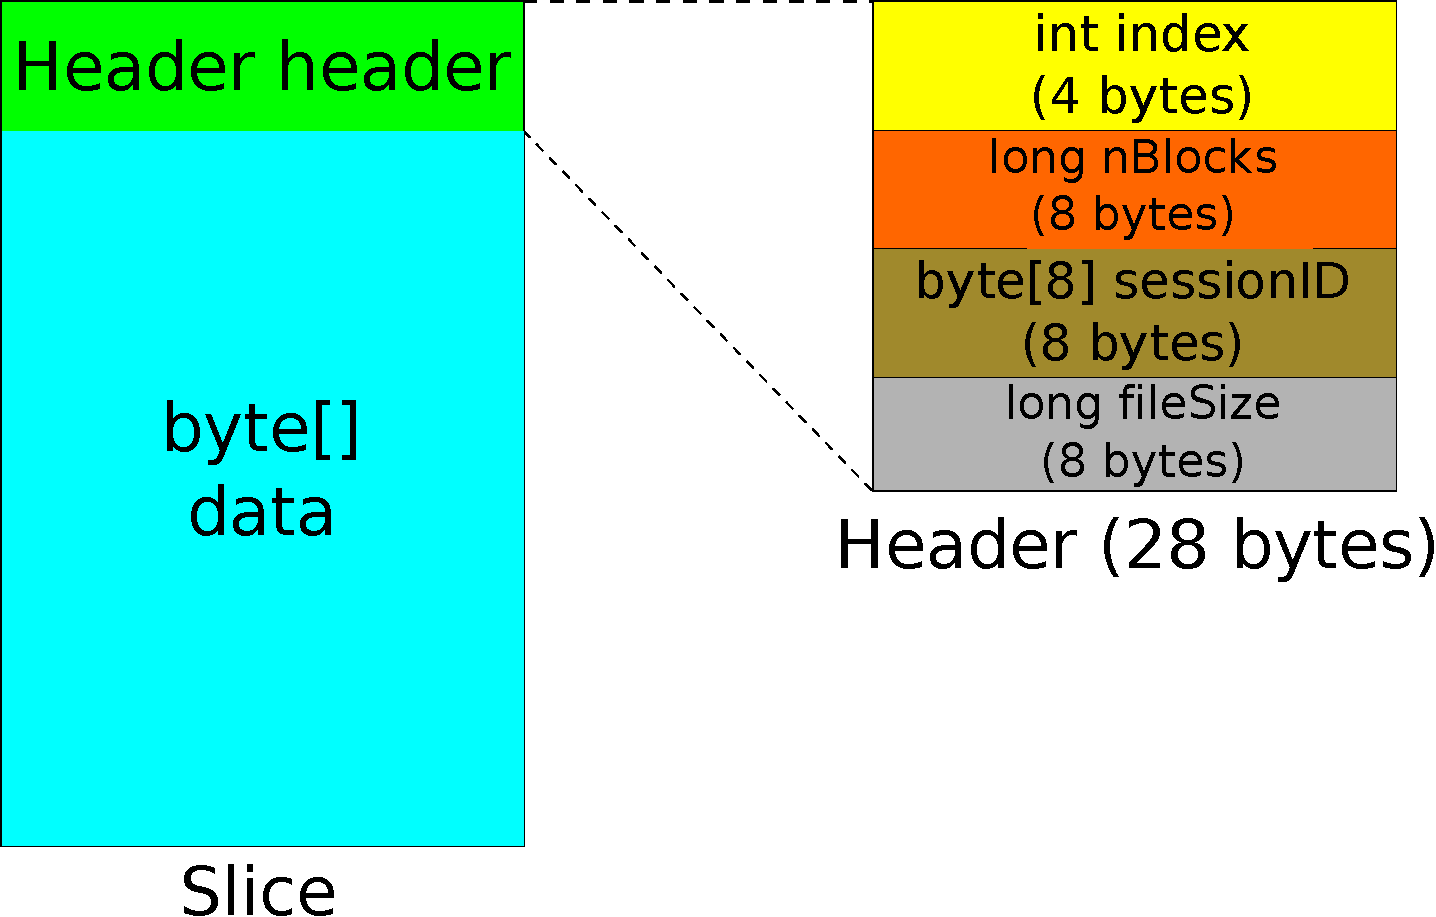
\includegraphics[scale=0.4]{Figures/Slice_Header_1}
  \decoRule
  \caption[\code{Slice} - \code{Header} (Versión 1)]{Esquema general de las clases \code{Slice} y \code{Header} (Versión 1)}
  \label{fig:Slice_Header_1}
\end{figure}

\begin{itemize}
  \item \keyword{\code{Slice}} -- Un objeto de clase \code{Slice} es uno de los fragmentos en los que un fichero original se ha dividido. Está formado por una cabecera (\code{Header}) y un array de \emph{bytes} en el que se almacena el contenido del segmento del fichero. (Figura~\ref{fig:Slice_Header_1}) \footnote{Debido al contexto del TFG, se ha decidido no usar UML para confeccionar los esquemas expuestos en este capítulo.}

  \item \keyword{\code{Header}} -- En esta clase se almacenan los metadatos de un objeto de clase \code{Slice}. Se guardan datos como un contador, el número total de fragmentos para un fichero, un ID para la sesión\footnote{En esta primera iteración de la aplicación, el ID para identificar la sesión es un resumen \emph{hash} del fichero.} y el tamaño original del fichero. (Figura~\ref{fig:Slice_Header_1})
\end{itemize}

También se han desarrollado otras clases con métodos para trocear y recomponer un fichero:

\begin{figure}[!htb]
  \centering
  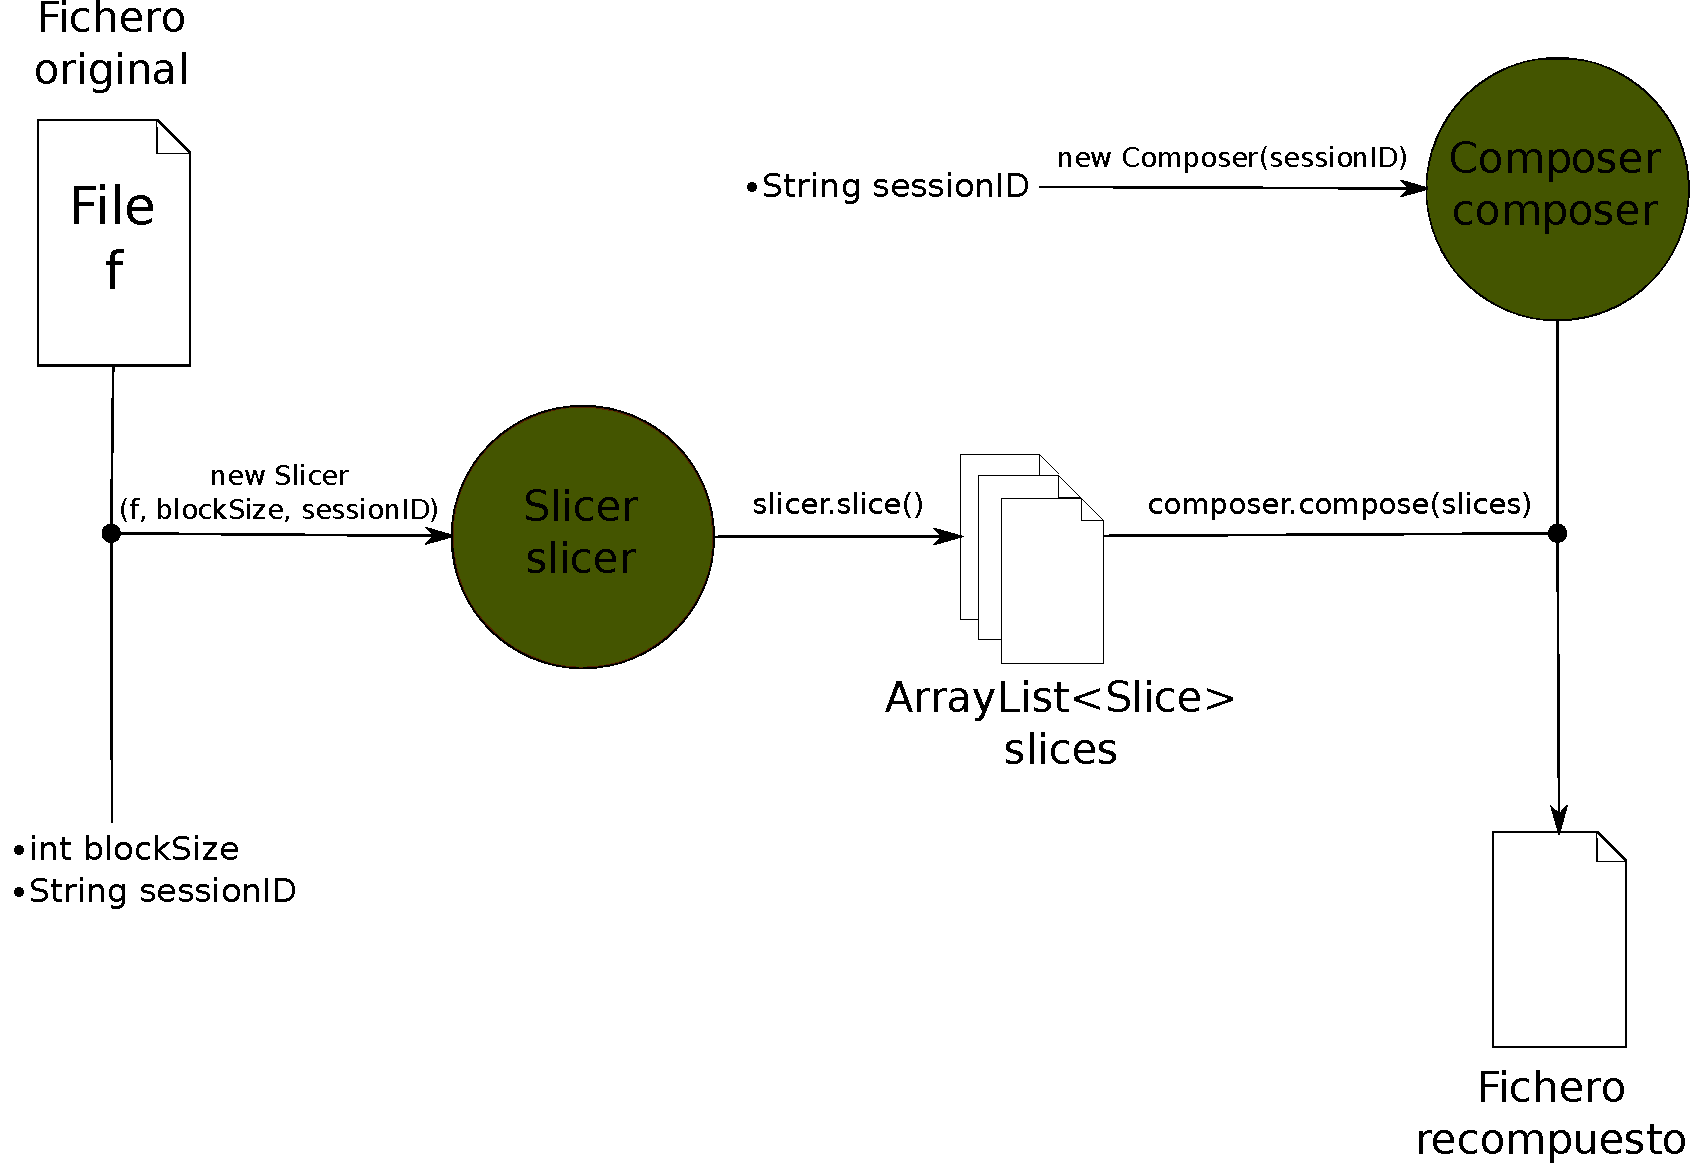
\includegraphics[scale=0.5]{Figures/Assembler}
  \decoRule
  \caption[\code{Slicer} - \code{Composer}]{Esquema general del funcionamiento de las clases \code{Slicer} y \code{Composer}}
  \label{fig:Assembler}
\end{figure}

\begin{itemize}
  \item \keyword{\code{Slicer}} -- Esta clase posee métodos para crear objetos de clase \code{Slice}. Recibe un fichero, un tamaño de bloque y un ID para identificar la sesión. Lee del fichero bloques del tamaño indicado hasta alcanzar el EOF y genera un \code{Slice} para cada uno de ellos, con una cabecera distinta. (Figura~\ref{fig:Assembler})

  \item \keyword{\code{Composer}} -- Esta clase, a través de un método, recibe un array de objetos de clase \code{Slice} y devuelve un fichero compuesto. Lee uno a uno los fragmentos que recibe, prestando especial atención a sus cabeceras y si detecta que alguno falta genera un log de errores. (Figura~\ref{fig:Assembler})
\end{itemize}

\subsection{Shatter II}

En esta segunda versión, el objetivo del prototipo es proporcionar confidencialidad a los objetos de clase \code{Slice}. Para llevarlo a cabo se han implementado las siguientes clases:

\begin{figure}[!htb]
  \centering
  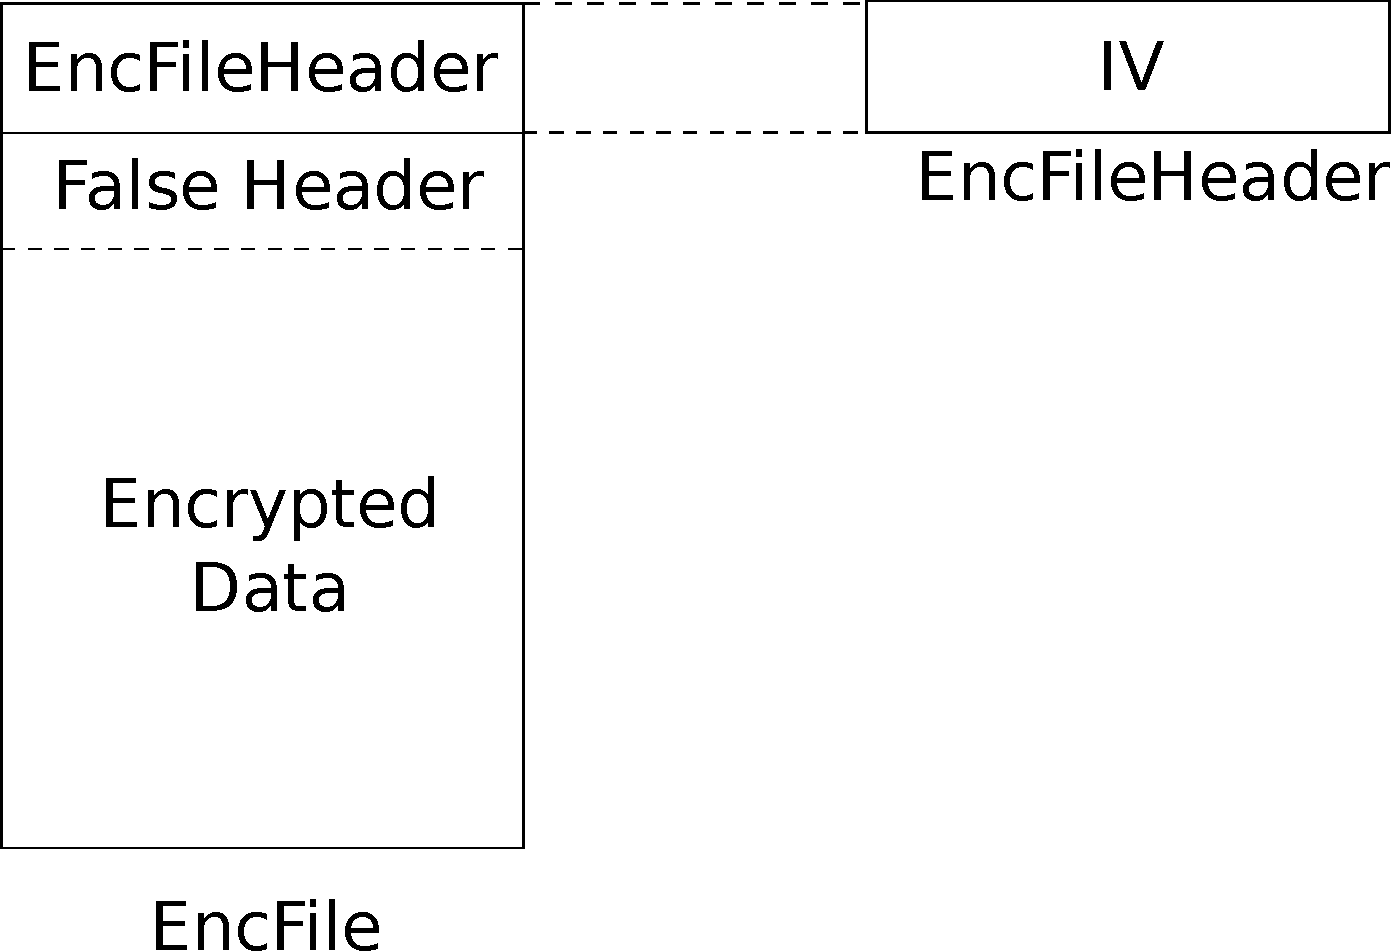
\includegraphics[scale=0.4]{Figures/EncFile_Header_1}
  \decoRule
  \caption[\code{EncFile} - \code{EncFileHeader} (Versión 1)]{Esquema general de las clases \code{EncFile} y \code{EncFileHeader} (Versión 1)}
  \label{fig:EncFile_Header_1}
\end{figure}

\begin{itemize}
  \item \keyword{\code{EncFile}} -- Viene a ser un objeto de clase \code{Slice} cifrado. A parte de los datos encriptados del \code{Slice}, también incluye una cabecera (\code{EncFileHeader}) con algunos datos importantes y una pseudocabecera (\code{FalseHeader}) con datos menores. (Figura~\ref{fig:EncFile_Header_1})

  \item \keyword{\code{EncFileHeader}} -- Esta cabecera se usa para almacenar algunos metadatos importantes como, en este caso, el vector de inicialización (IV) que se ha usado en el cifrado del objeto \code{Slice}. (Figura~\ref{fig:EncFile_Header_1})

  \item \keyword{\code{KeyFile}} -- Esta clase se utiliza para almacenar la clave simétrica que se ha utilizado para crear los objetos de clase \code{EncFile}.
\end{itemize}

Además de estas clases, se han creado otras clases que aportan los métodos necesarios para cifrar los fragmentos:

\begin{figure}[!htb]
  \centering
  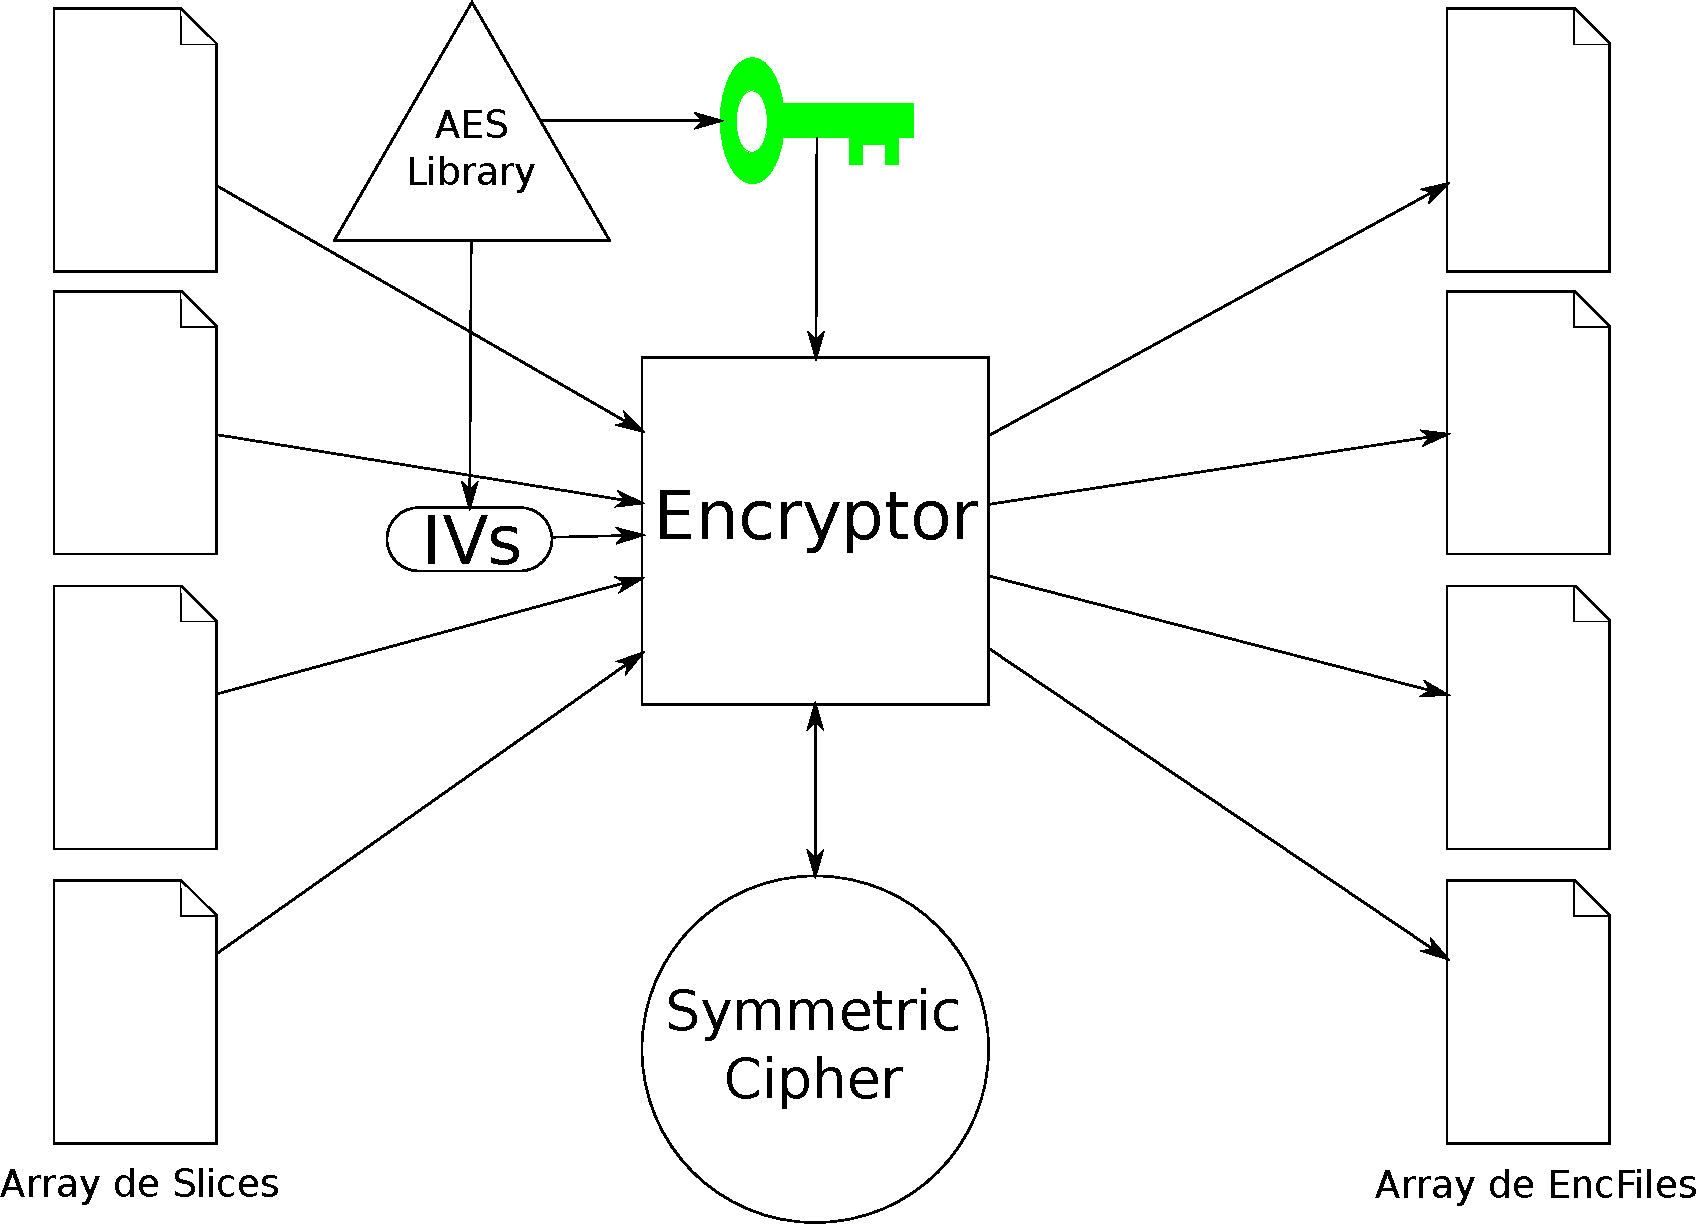
\includegraphics[scale=0.5]{Figures/Encryptor}
  \decoRule
  \caption[\code{Encryptor}]{Esquema general del funcionamiento de la clase \code{Encryptor}}
  \label{fig:Encryptor}
\end{figure}

\begin{figure}[!htb]
  \centering
  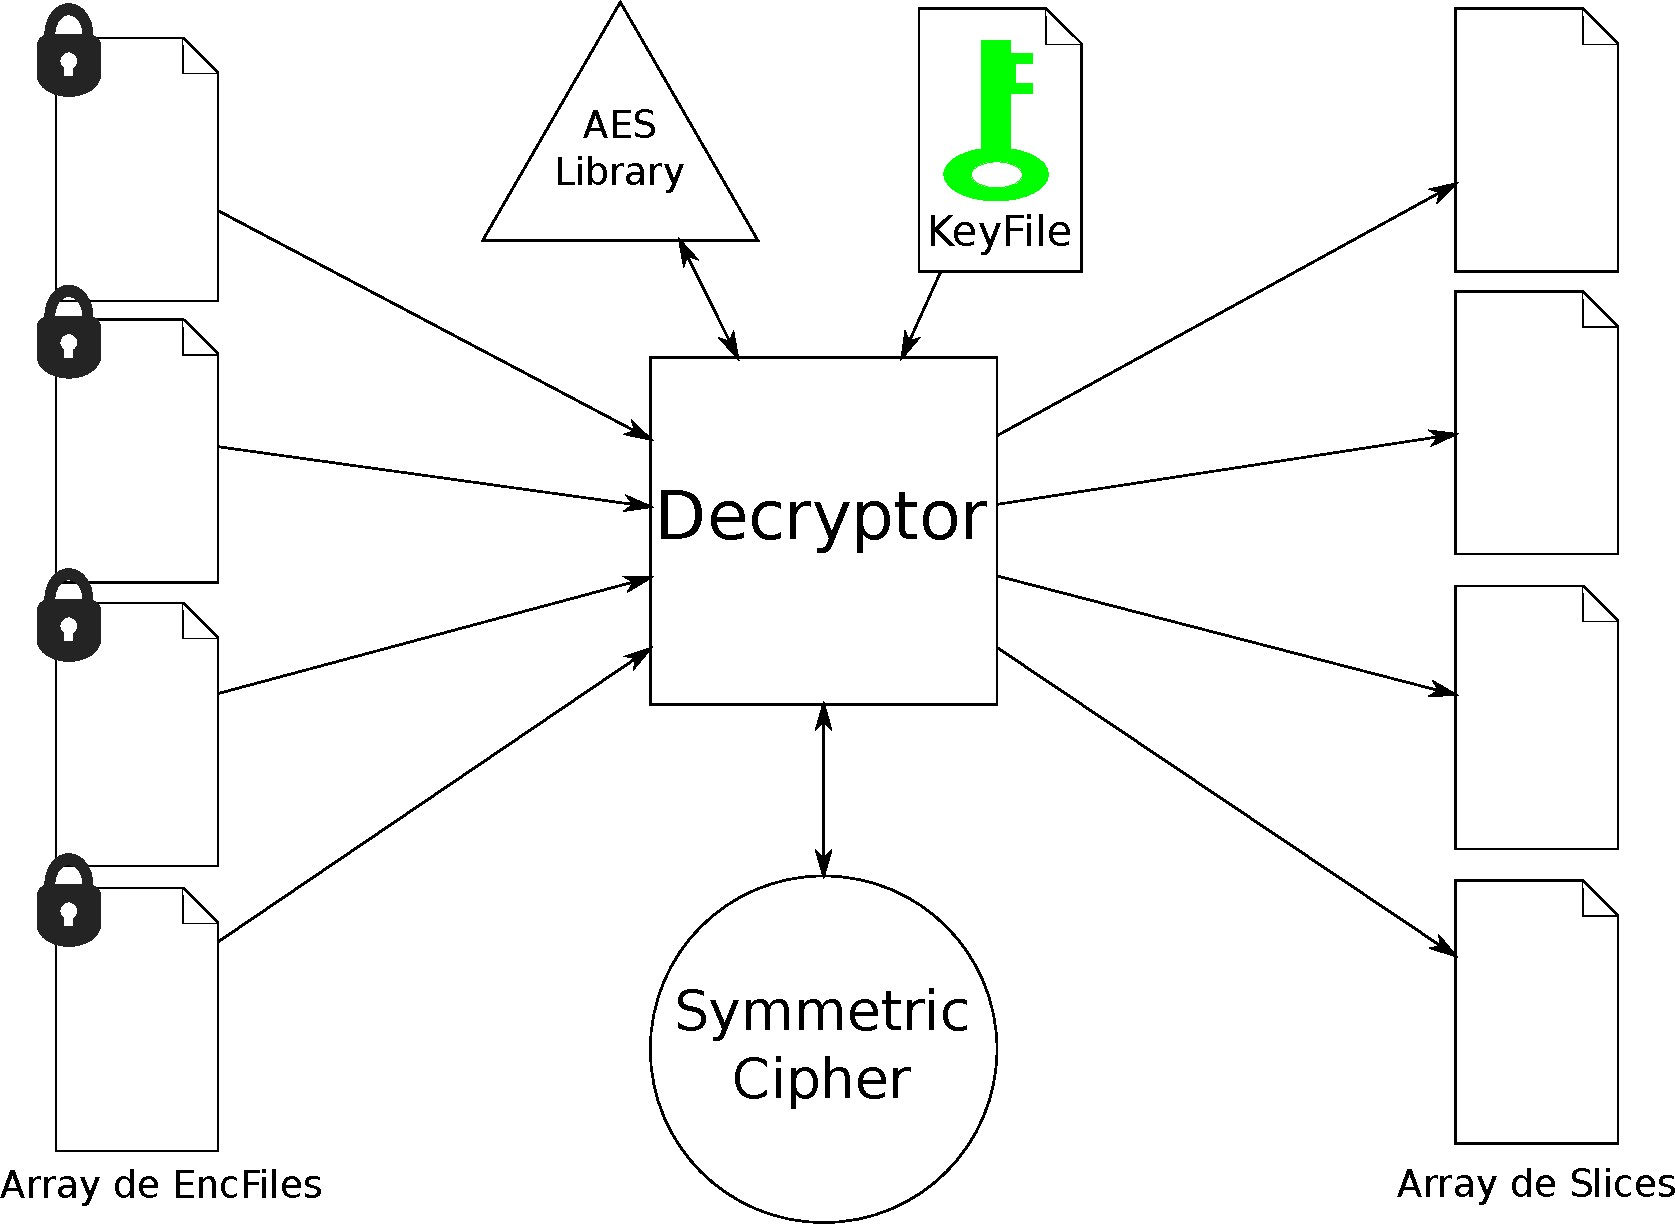
\includegraphics[scale=0.5]{Figures/Decryptor}
  \decoRule
  \caption[\code{Decryptor}]{Esquema general del funcionamiento de la clase \code{Decryptor}}
  \label{fig:Decryptor}
\end{figure}

\begin{itemize}
  \item \keyword{\code{AESLibrary}} -- Básicamente, una clase que se encarga de generar de manera aleatoria y segura claves simétricas y vectores de inicialización.

  \item \keyword{\code{SymmetricCipher}} -- Esta es la clase que se encarga de hacer la parte más importante en cuanto a la confidencialidad. Una vez que ha sido inicializada con una clave simétrica, genera textos cifrados a partir de texto plano y un IV. Igualmente, puede llevar a cabo el proceso inverso.

  \item \keyword{\code{Encryptor}} -- Esta clase, en conjunto con las dos anteriores, es la encargada de generar los objetos de clase \code{EncFile}. Genera de manera aleatoria y segura una clave simétrica para un algoritmo establecido y, con ella, inicializa una instancia de la clase \code{SymmetricCipher}. A continuación se le pasa un array de objetos de clase \code{Slice} del cual genera un array de objetos de clase \code{EncFile}, que es el que devuelve a través de un método. (Figura~\ref{fig:Encryptor})

  \item \keyword{\code{Decryptor}} -- La contraparte de la clase \code{Encryptor}. Realiza el proceso inverso y devuelve un array de objetos de clase \code{Slice} a partir de uno de objetos de clase \code{EncFile}. (Figura~\ref{fig:Decryptor})
\end{itemize}

\subsection{Shatter III}

El objetivo en esta tercera iteración es el de proporcionar integridad y autenticación a las clases ya implementadas, al igual que confidencialidad a la clave simétrica que se utiliza para generarlas. Para lograrlo, se han implementado algunas clases nuevas:

\begin{itemize}
  \item \keyword{\code{EncKeyFile}} -- Esta clase almacena la clave simétrica protegida mediante cifrado asimétrico usando la clave pública del destinatario del mensaje, con lo que se logra la confidencialidad de la clave entre los usuarios. Tiene una cabecera (\code{EncKeyFileHeader}) en la que se guardan algunos datos importantes.

  \item \keyword{\code{EncKeyFileHeader}} -- La cabecera de un objeto de clase \code{EncKeyFile}. En ella se almacena una HMAC cifrada de la clave simétrica.

  \item \keyword{\code{Signature}} -- Básicamente una clase para contener una HMAC.

  \item \keyword{\code{SecureSignature}} -- Contiene la HMAC comentada antes pero cifrada usando una clave asimétrica. De esta forma también le damos confidencialidad a la firma.
\end{itemize}

Para poder llevar a cabo el cifrado asimétrico se han desarrollado otras clases:

\begin{figure}[!htb]
  \centering
  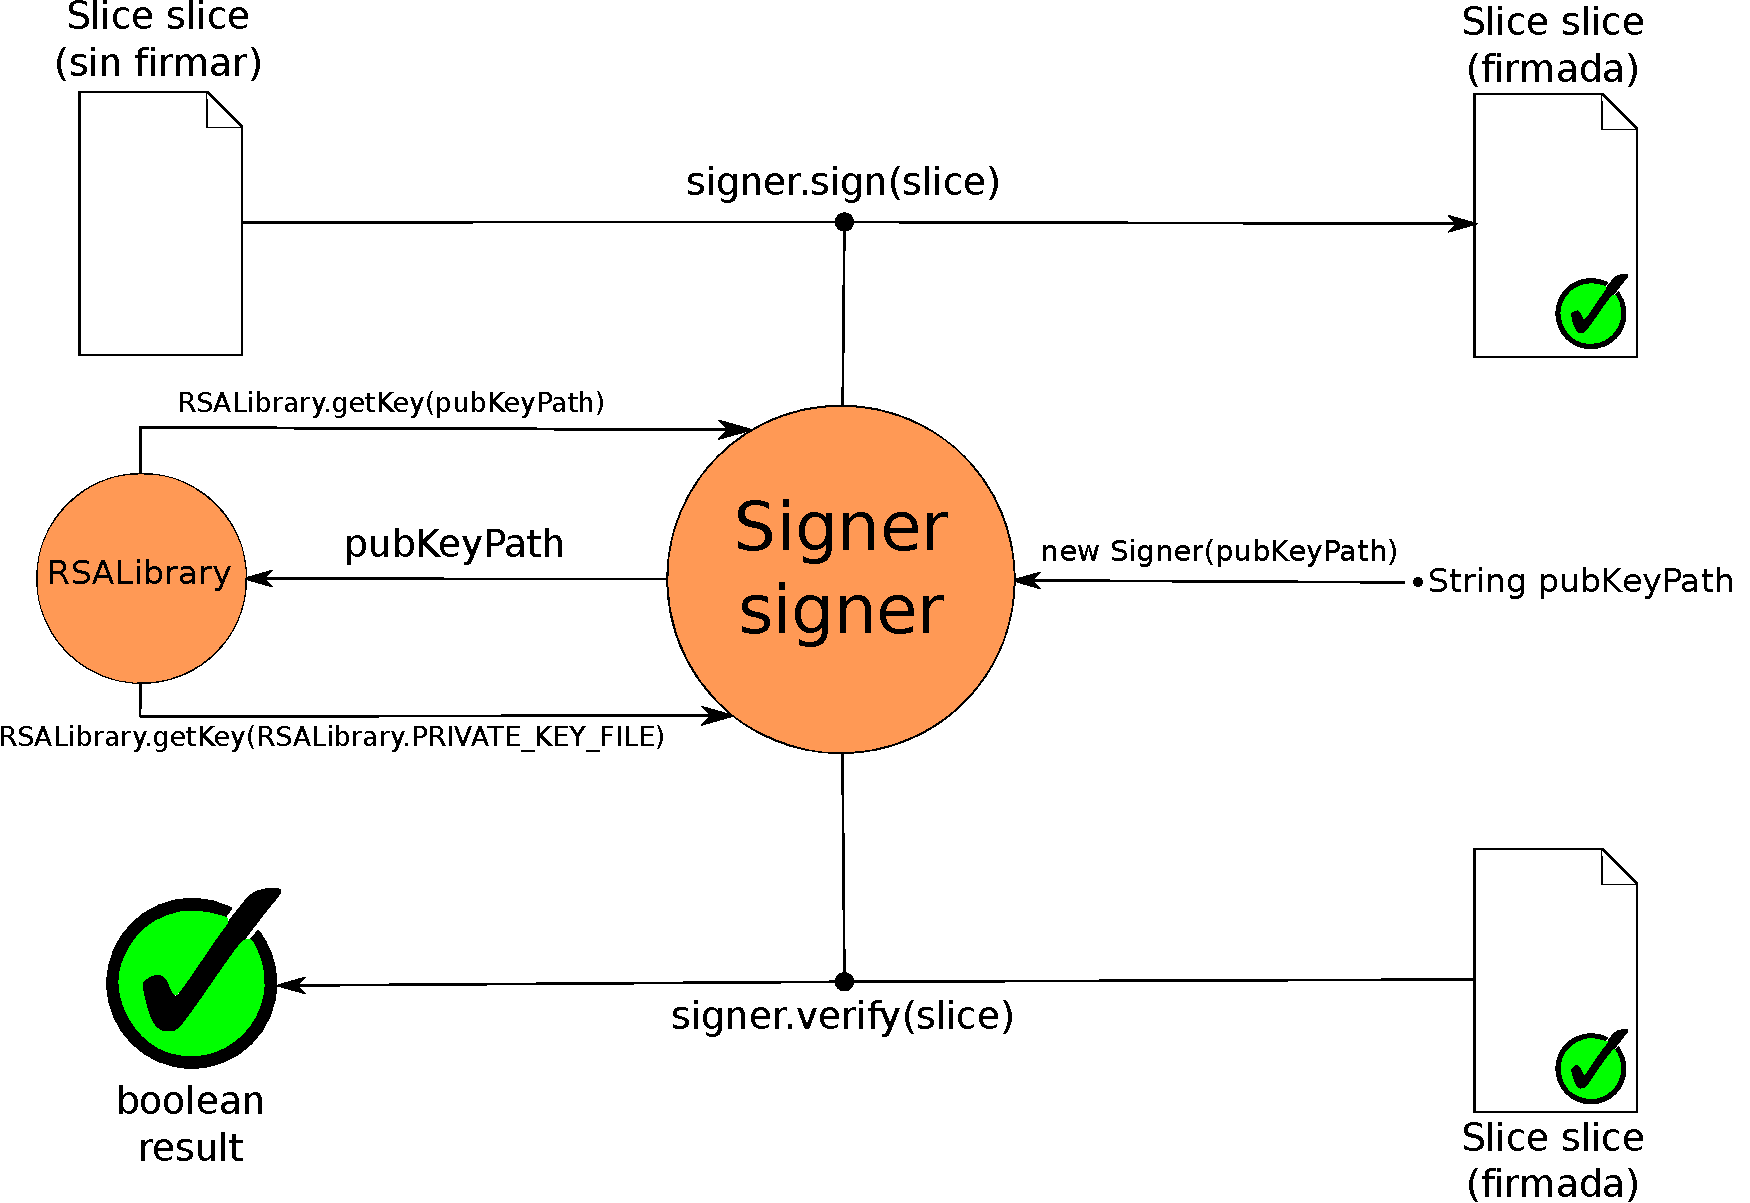
\includegraphics[scale=0.5]{Figures/Signer_1}
  \decoRule
  \caption[\code{Signer} (Versión 1)]{Esquema general del funcionamiento de la clase \code{Signer} (Versión 1)}
  \label{fig:Signer_1}
\end{figure}

\begin{itemize}
  \item \keyword{\code{RSALibrary}} -- Esta clase es la encargada de generar un par de claves asimétricas, de escribirlas y leerlas de un fichero, de cifrar un texto plano y de descifrar uno cifrado.

  \item \keyword{\code{Signer}} -- La clase que se encarga de recibir objetos de clase \code{Slice}, \code{EncFile}, \code{KeyFile} y demás y devolverlos firmados. Asimismo, se encarga de comprobar las firmas de todas estas clases para preservar la autenticidad de la información que portan. (Figura~\ref{fig:Signer_1})

  \item \keyword{\code{RSAPSS}} -- Esta clase incorpora todos los métodos necesarios para generar, a partir de un texto plano, un texto codificado y firmado usando el algoritmo RSASSA-PSS. También realiza el proceso inverso y puede verificar las firmas.
\end{itemize}

En este prototipo se ha añadido una firma a varias de las clases que ya estaban implementadas:

\begin{figure}[!htb]
  \centering
  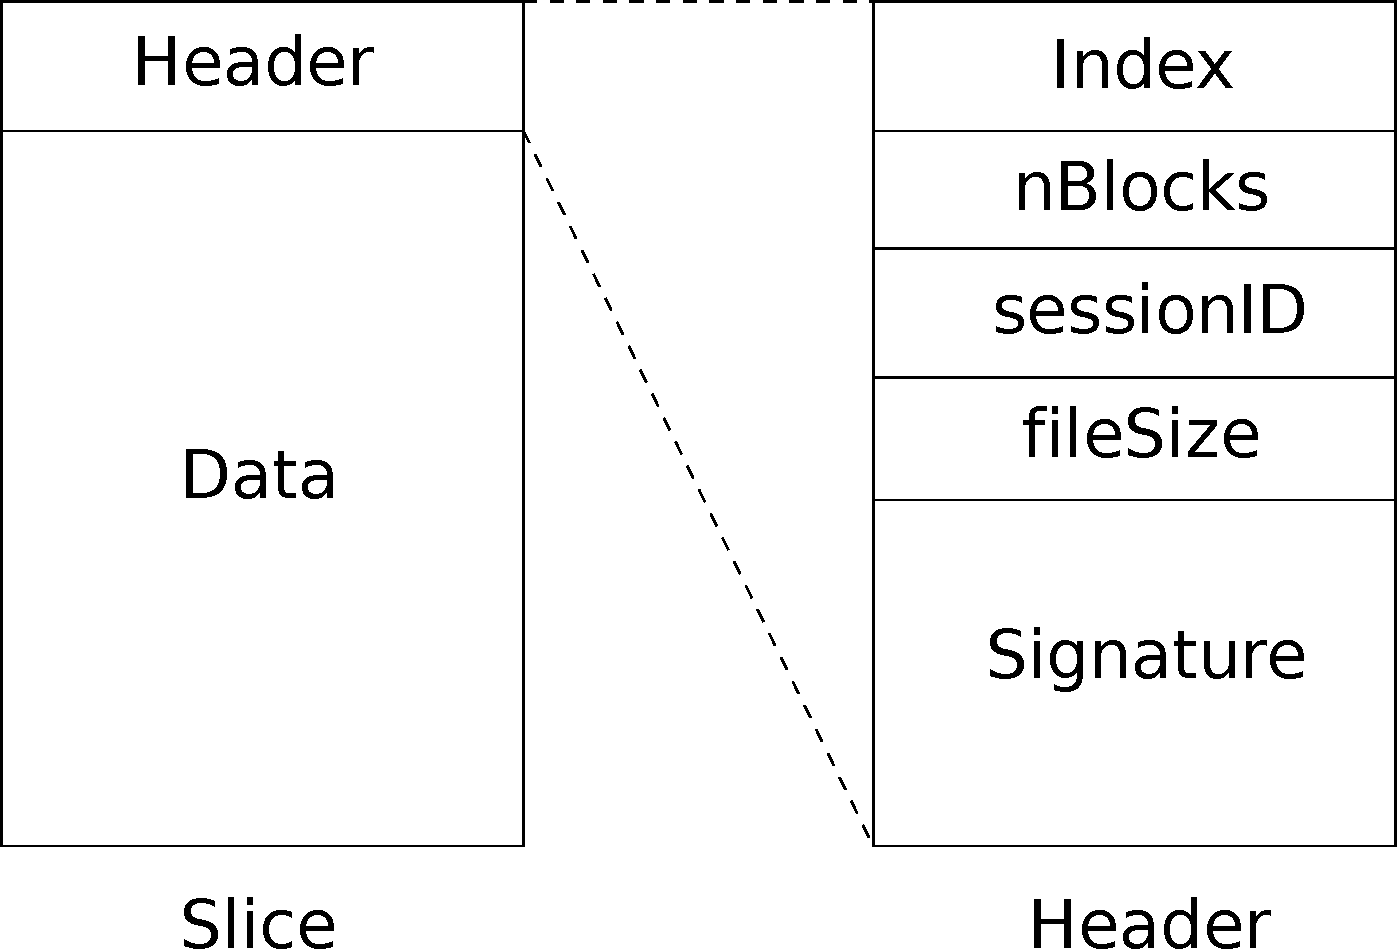
\includegraphics[scale=0.4]{Figures/Slice_Header_2}
  \decoRule
  \caption[\code{Slice} - \code{Header} (Versión final)]{Esquema general de las clases \code{Slice} y \code{Header} (Versión final)}
  \label{fig:Slice_Header_2}
\end{figure}

\begin{figure}[!htb]
  \centering
  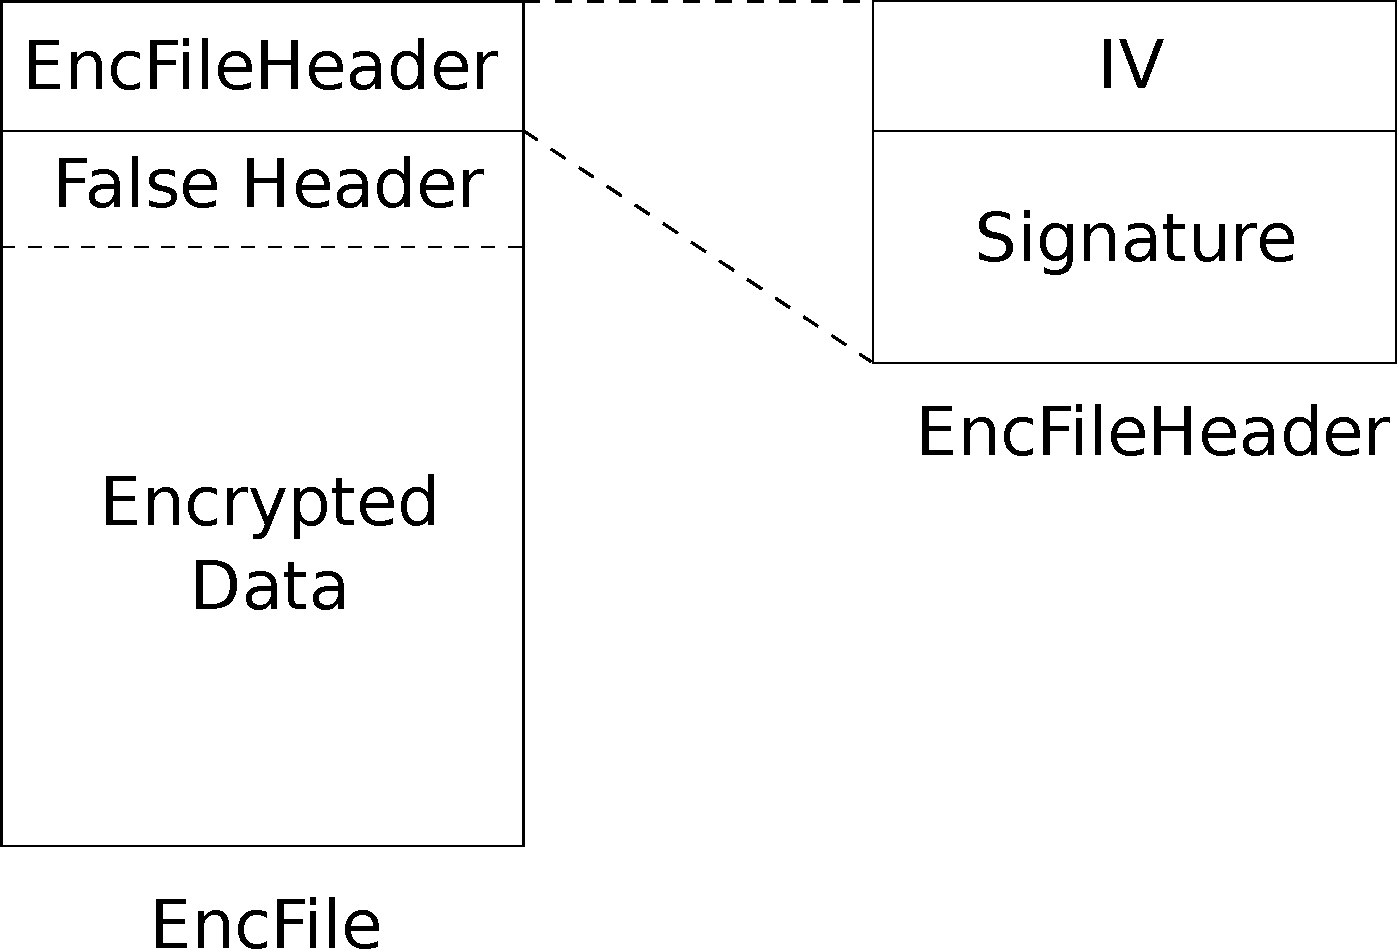
\includegraphics[scale=0.4]{Figures/EncFile_Header_2}
  \decoRule
  \caption[\code{EncFile} - \code{EncFileHeader} (Versión final)]{Esquema general de las clases \code{EncFile} y \code{EncFileHeader} (Versión final)}
  \label{fig:EncFile_Header_2}
\end{figure}

\begin{itemize}
  \item A la clase \code{Slice} se le ha añadido en la cabecera una firma, que otorga integridad y autenticación a los datos que lleva. (Figura~\ref{fig:Slice_Header_2})

  \item A la clase \code{EncFile} se le ha añadido también una firma, esta vez para darle la integridad y la autenticación al IV que se encuentra en su cabecera. (Figura~\ref{fig:EncFile_Header_2})

  \item La clase \code{KeyFile} tiene una firma de la clave simétrica.
\end{itemize}

Además de las clases mencionadas anteriormente, también se han desarrollado otras clases funcionales:

\begin{itemize}
  \item \keyword{\code{RandomString}} -- Esta clase posee un método que devuelve un \code{String} aleatorio de 8 caracteres.

  \item \keyword{\code{FileIO}} -- Esta clase tiene métodos para escribir y leer los distintos ficheros que intervienen en la aplicación.

  \item \keyword{\code{Bytes}} -- Tiene implementados varios métodos para hacer operaciones con arrays de \emph{bytes}.
\end{itemize}

\subsection{Shatter IV}

Este último prototipo está desarrollado como una aplicación en Android. El objetivo de este prototipo es hacer uso de varias herramientas que posee Android para que la aplicación funcione correctamente. Para ello se han creado nuevas clases:

\begin{itemize}
  \item \keyword{\code{KeyStoreHandler}} -- Esta clase se usa para realizar todas las operaciones necesarias con el \emph{Keystore} de Android (Véase~\ref{Keystore}). Se encarga de almacenar las claves, recuperarlas, usarlas para encriptar, firmar, etc.

  \item \keyword{\code{HTTPClient}} -- Un cliente HTTP muy sencillo que únicamente realiza peticiones GET.

  \item \keyword{\code{ExternalStorage}} -- Esta clase se encarga de interactuar con el \emph{External Storage} de Android. Incorpora algunos métodos para conseguir \emph{paths}, descriptores de fichero o crear directorios.
\end{itemize}

Para que los usuarios puedan enviar sus mensajes, se ha dispuesto un servidor HTTP bastante sencillo al que los usuarios pueden subir sus mensajes. Gracias a la clase \code{HTTPClient}, el destinatario puede bajarse los fragmentos de un mensaje.

\begin{figure}[!htb]
  \centering
  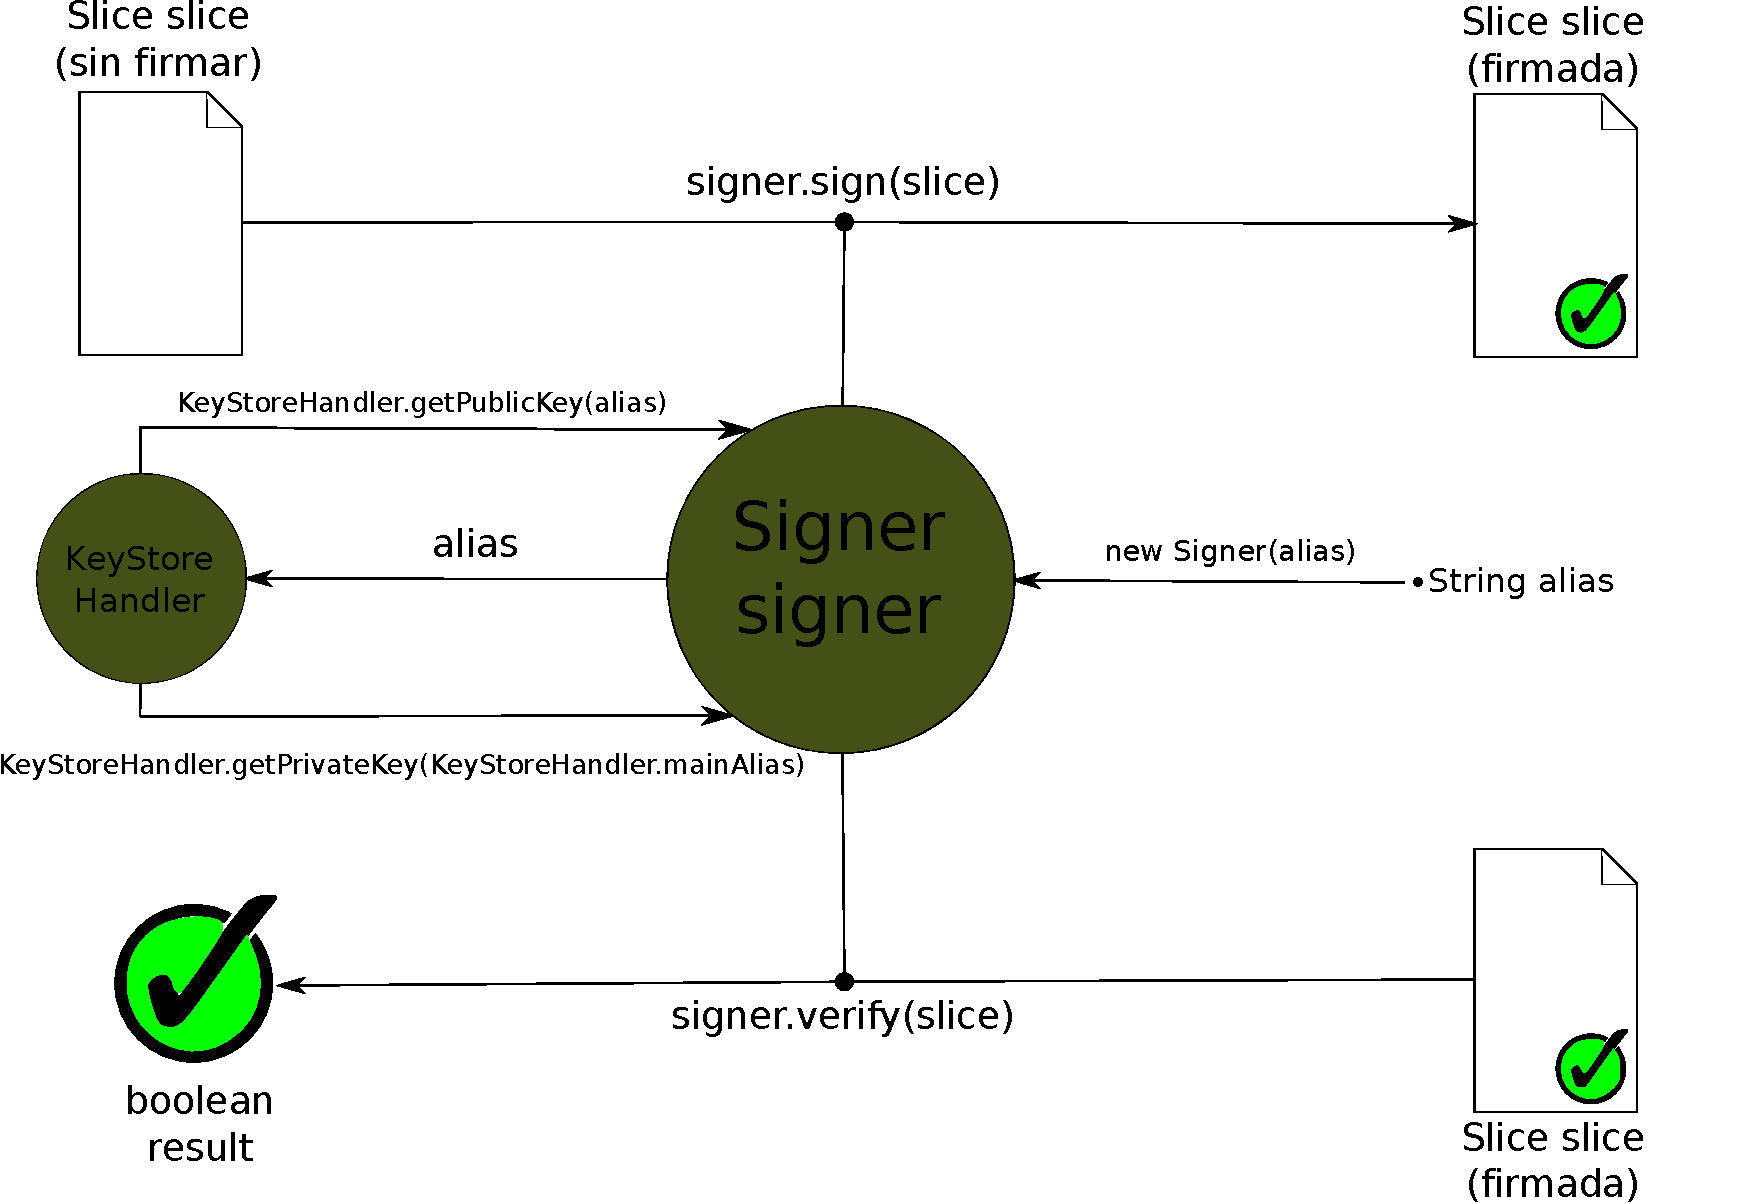
\includegraphics[scale=0.5]{Figures/Signer_2}
  \decoRule
  \caption[\code{Signer} (Versión final)]{Esquema general del funcionamiento de la clase \code{Signer} (Versión final)}
  \label{fig:Signer_2}
\end{figure}

El uso del \emph{Keystore} de Android obliga a utilizar las claves que se almacenan en él usando unos métodos específicos. Debido a ello, algunas clases ya creadas (Como \code{RSALibrary} o \code{RSAPSS}) se sustituyen por métodos específicos que se implementan en la clase \code{KeyStoreHandler}. (Figura~\ref{fig:Signer_2})

El ID que aparece en las cabeceras de la clase \code{Slice} se sustituye por un \code{String} aleatorio que genera la clase \code{RandomString}. Este cambio se debe a que el resumen \emph{hash} que se usaba anteriormente queda en desuso al añadir la firma a estas clases. Además, este ID aleatorio identifica a todos los objetos de clase \code{Slice} que pertenecen a un mismo mensaje.

El esquema general de la aplicación se puede dividir en dos: Una primera parte se encarga de la división y cifrado del fichero (Figura~\ref{fig:abstractA}). La otra se encarga de descargar del servidor los fragmentos cifrados y recomponer el fichero original (Figura~\ref{fig:abstractB}).

\begin{figure}[!htb]
  \centering
  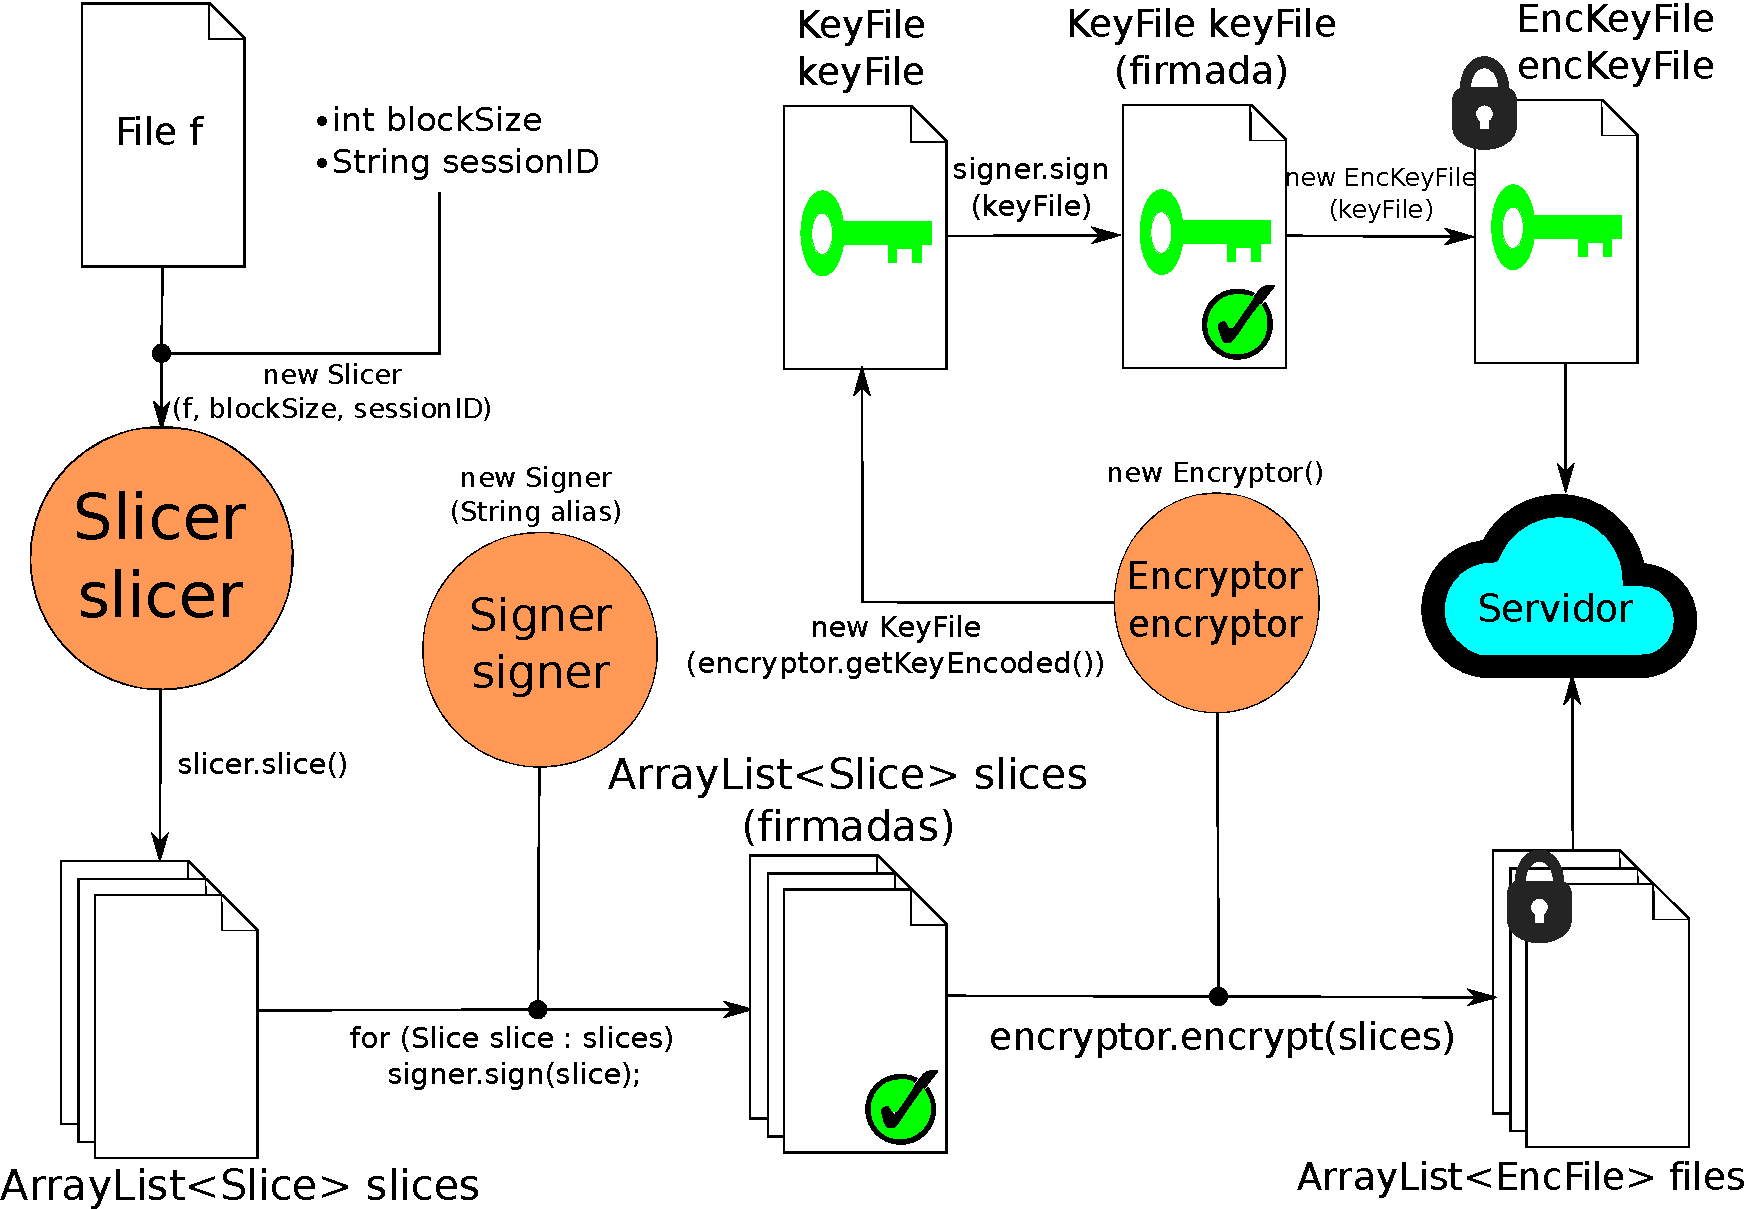
\includegraphics[scale=0.5]{Figures/abstractA}
  \decoRule
  \caption[\code{SliceEncrypt}]{Esquema general de la clase \code{SliceEncrypt}, la primera parte en el proceso de comunicación de la aplicación}
  \label{fig:abstractA}
\end{figure}

\begin{figure}[!htb]
  \centering
  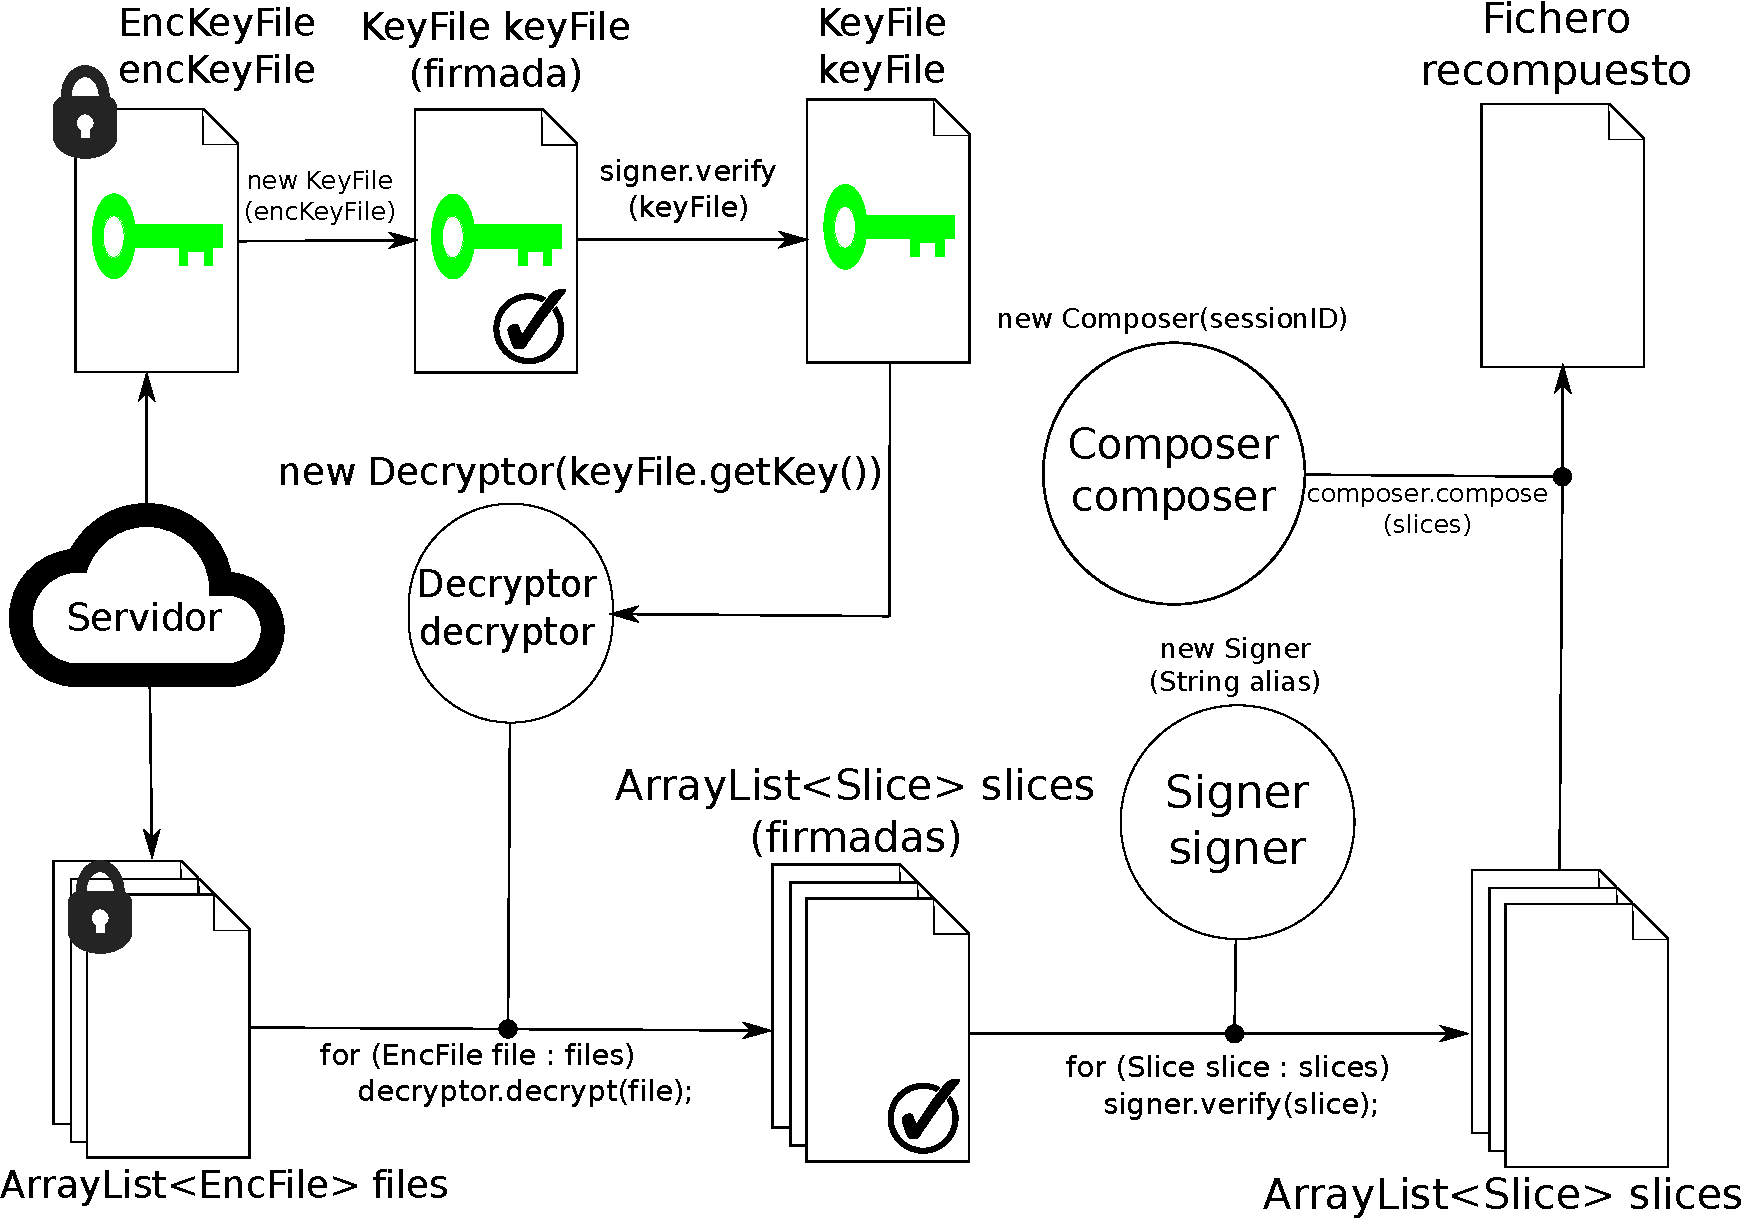
\includegraphics[scale=0.5]{Figures/abstractB}
  \decoRule
  \caption[\code{DecryptCompose}]{Esquema general de \code{DecryptCompose}, la parte final en el proceso de comunicación de la aplicación}
  \label{fig:abstractB}
\end{figure}

%-------------------------------------------------------------------------------

\section{Tiempo dedicado}

El desarrollo de cada prototipo ha necesitado un tiempo de trabajo distinto. En esta sección se detalla el número de horas dedicado a cada uno de ellos:

\begin{itemize}
  \item El primer prototipo, al tratarse de un esquema bastante sencillo, no ha supuesto un número de horas excesivo. El desarrollo de este prototipo se finalizó a las dos semanas de iniciar el proyecto, habiendo dedicado una media de dos horas diarias (28 horas).

  \item El segundo prototipo ha supuesto no solo tiempo de desarrollo, también ha necesitado tiempo de investigación para elegir el algoritmo más adecuado para el proyecto. Para este prototipo se dedicó, a partir de la finalización del prototipo anterior, dos semanas de desarrollo y una de investigación, dedicando una media de dos horas diarias (42 horas).

  \item El tercer prototipo ha necesitado una primera parte de investigación para elegir el algoritmo de cifrado asimétrico y firma adecuados y luego una parte de desarrollo. El desarrollo de este prototipo ha requerido, a partir de la finalización del prototipo anterior, dos semanas de investigación y cuatro de desarrollo, dedicando una media de dos horas diarias (84 horas).

  \item El cuarto prototipo, al tratarse de una migración a otra plataforma, no debería haber supuesto mucho tiempo de trabajo. Sin embargo se ha dedicado más tiempo debido a los problemas que se detallan en el Capítulo~\ref{Chapter5.2}. Esta fase ha requerido una primera semana de investigación para encontrar la mejor forma de realizar la migración, y cinco semanas de desarrollo para llevarlo a cabo, dedicando una media de dos horas diarias (84 horas).
\end{itemize}

En total, el desarrollo del proyecto ha conllevado aproximadamente 238 horas de trabajo, habiendo invertido más tiempo en el desarrollo que en la investigación.

% Chapter 5: Results

\chapter{Resultados} % Main chapter title

\label{Chapter5} % Reference

%-------------------------------------------------------------------------------

\section{Ejemplos de uso de la aplicación}

%En esta sección se va a poner un ejemplo de como un usuario utilizaría la aplicación ya descargada en su terminal móvil.
Esta sección muestra un ejemplo de uso completo de la aplicación, pasando por los prerrequisitos, el cifrado de un fichero y la descarga de un mensaje.

\begin{figure}[!htb]
  \centering
  
\includegraphics[scale=0.2]{Figures/launcher}
  \decoRule
  \caption[Shatter (Icono)]{Icono de la aplicación Shatter}
  \label{fig:launcher}
\end{figure}

\subsection{Prerrequisitos}

Al tratarse de una aplicación Android, es necesario el uso de un dispositivo que utilice el sistema operativo Android (Véase~\ref{Android}), específicamente la versión 6 (Marshmallow) o una superior.

También es necesario dar permisos de escritura en el almacenamiento del dispositivo, ya que la aplicación realiza operaciones de escritura y lectura.

\subsection{Añadir contactos}

Al abrir la aplicación por primera vez se genera un par de claves asimétricas, una pública y otra privada. En la pantalla principal, al no disponer de ningún contacto, solo se puede ver un campo de texto, un botón para seleccionar un fichero y un botón para añadir usuarios. (Figura~\ref{fig:home})

\begin{figure}[!htb]
  \centering
  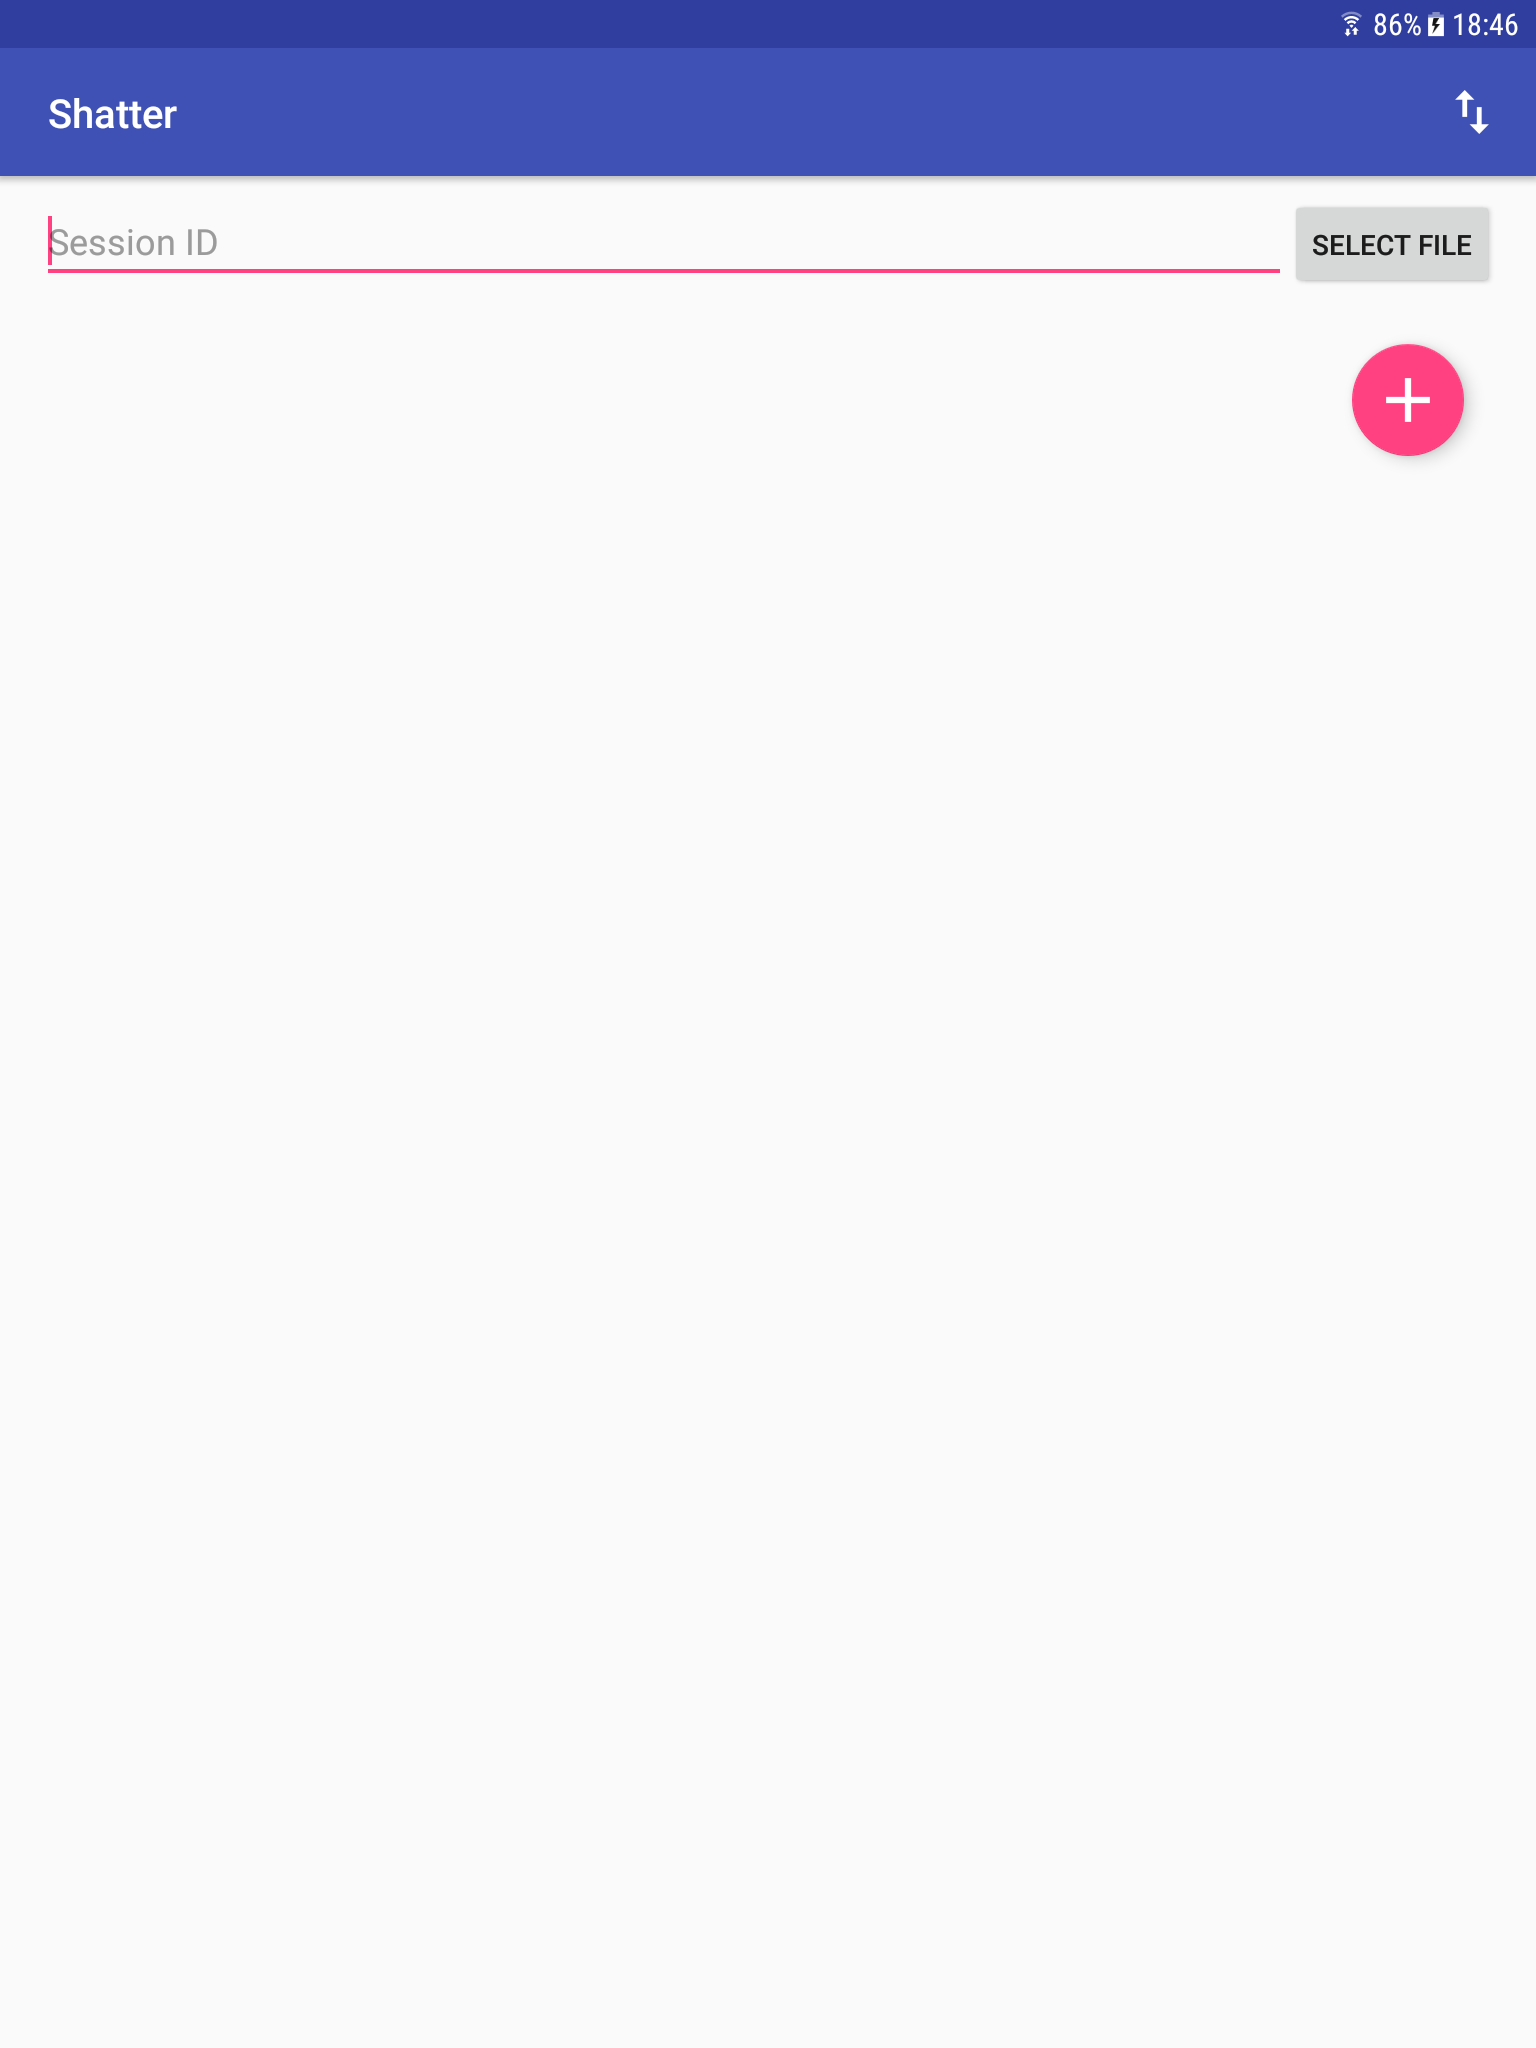
\includegraphics[scale=0.4]{Figures/home}
  \decoRule
  \caption[Shatter (Home)]{Pantalla principal de la aplicación}
  \label{fig:home}
\end{figure}

El primer objetivo es añadir algún usuario a la lista de contactos. Lo primero que hay que hacer es exportar la clave pública previamente generada haciendo uso del icono que se encuentra en la barra superior de la pantalla principal. (Figura~\ref{fig:export})

\begin{figure}[!htb]
  \centering
  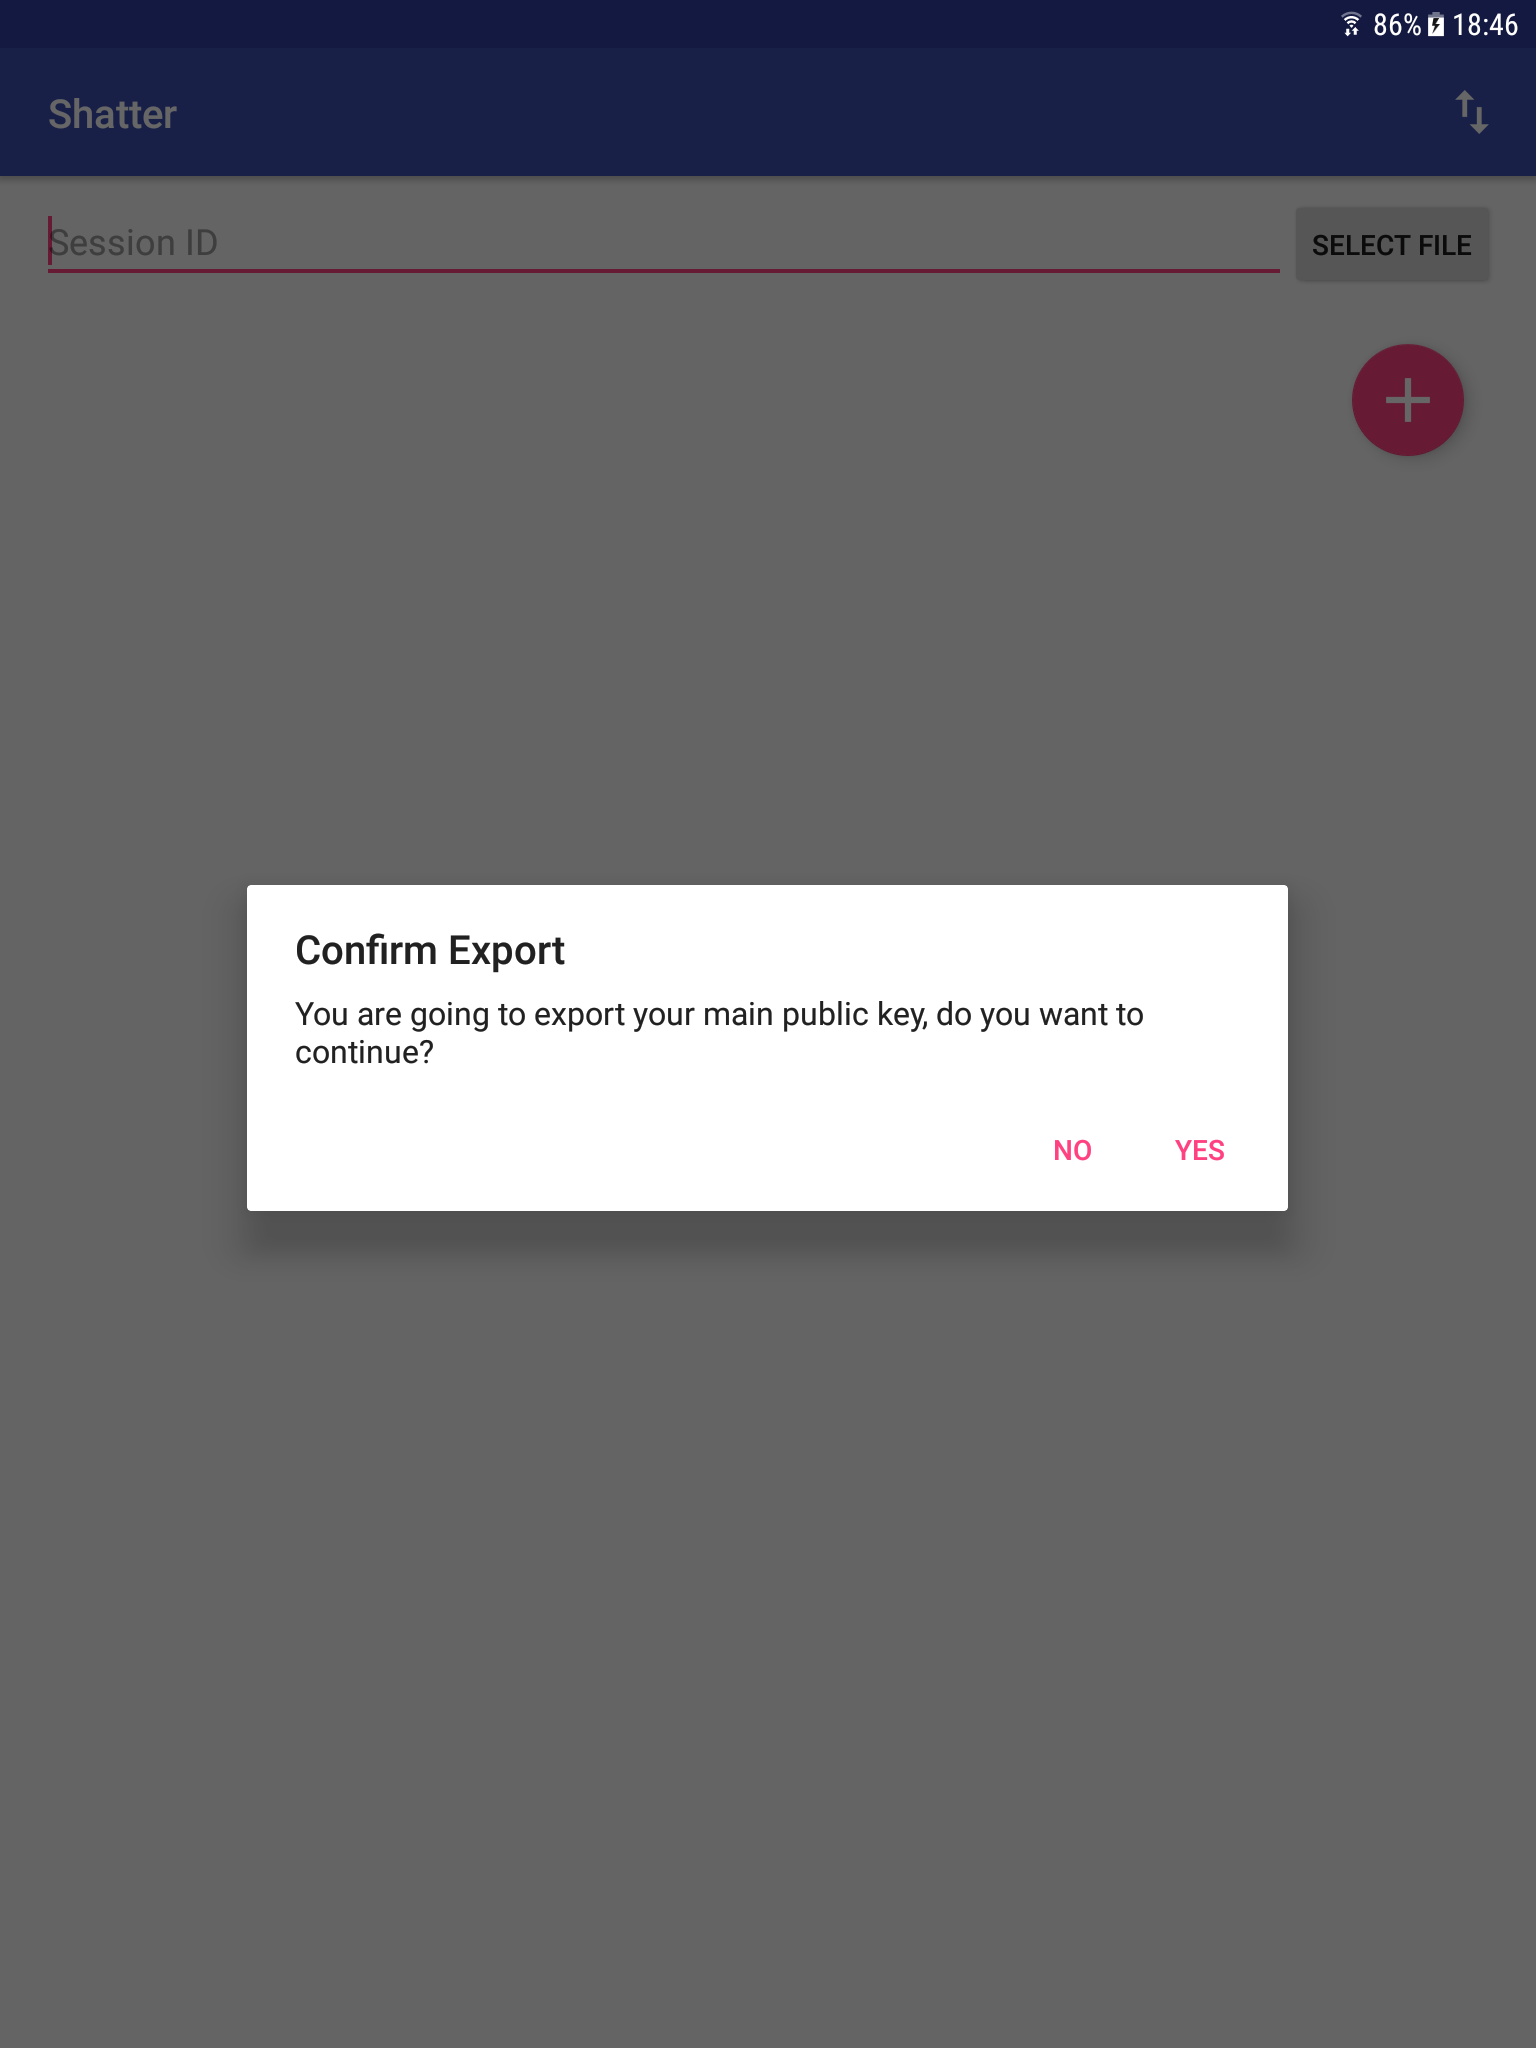
\includegraphics[scale=0.4]{Figures/export}
  \decoRule
  \caption[Shatter (Exportar clave pública)]{Mensaje de advertencia al exportar la clave pública}
  \label{fig:export}
\end{figure}

Al confirmar, se genera un certificado el cual contiene la clave pública antes generada en la ruta \path{Shatter/certs/main.crt}. \footnote{El directorio principal de la aplicación se encuentra en el almacenamiento externo del terminal y es accesible mediante un explorador de archivos.}

Para añadir a un contacto se dispone de un botón en la esquina inferior derecha de la pantalla principal, el cual abre una nueva pantalla en la que se puede especificar un alias (nombre de usuario) y un certificado con la clave pública del nuevo usuario. (Figura~\ref{fig:import})

\begin{figure}[!htb]
  \centering
  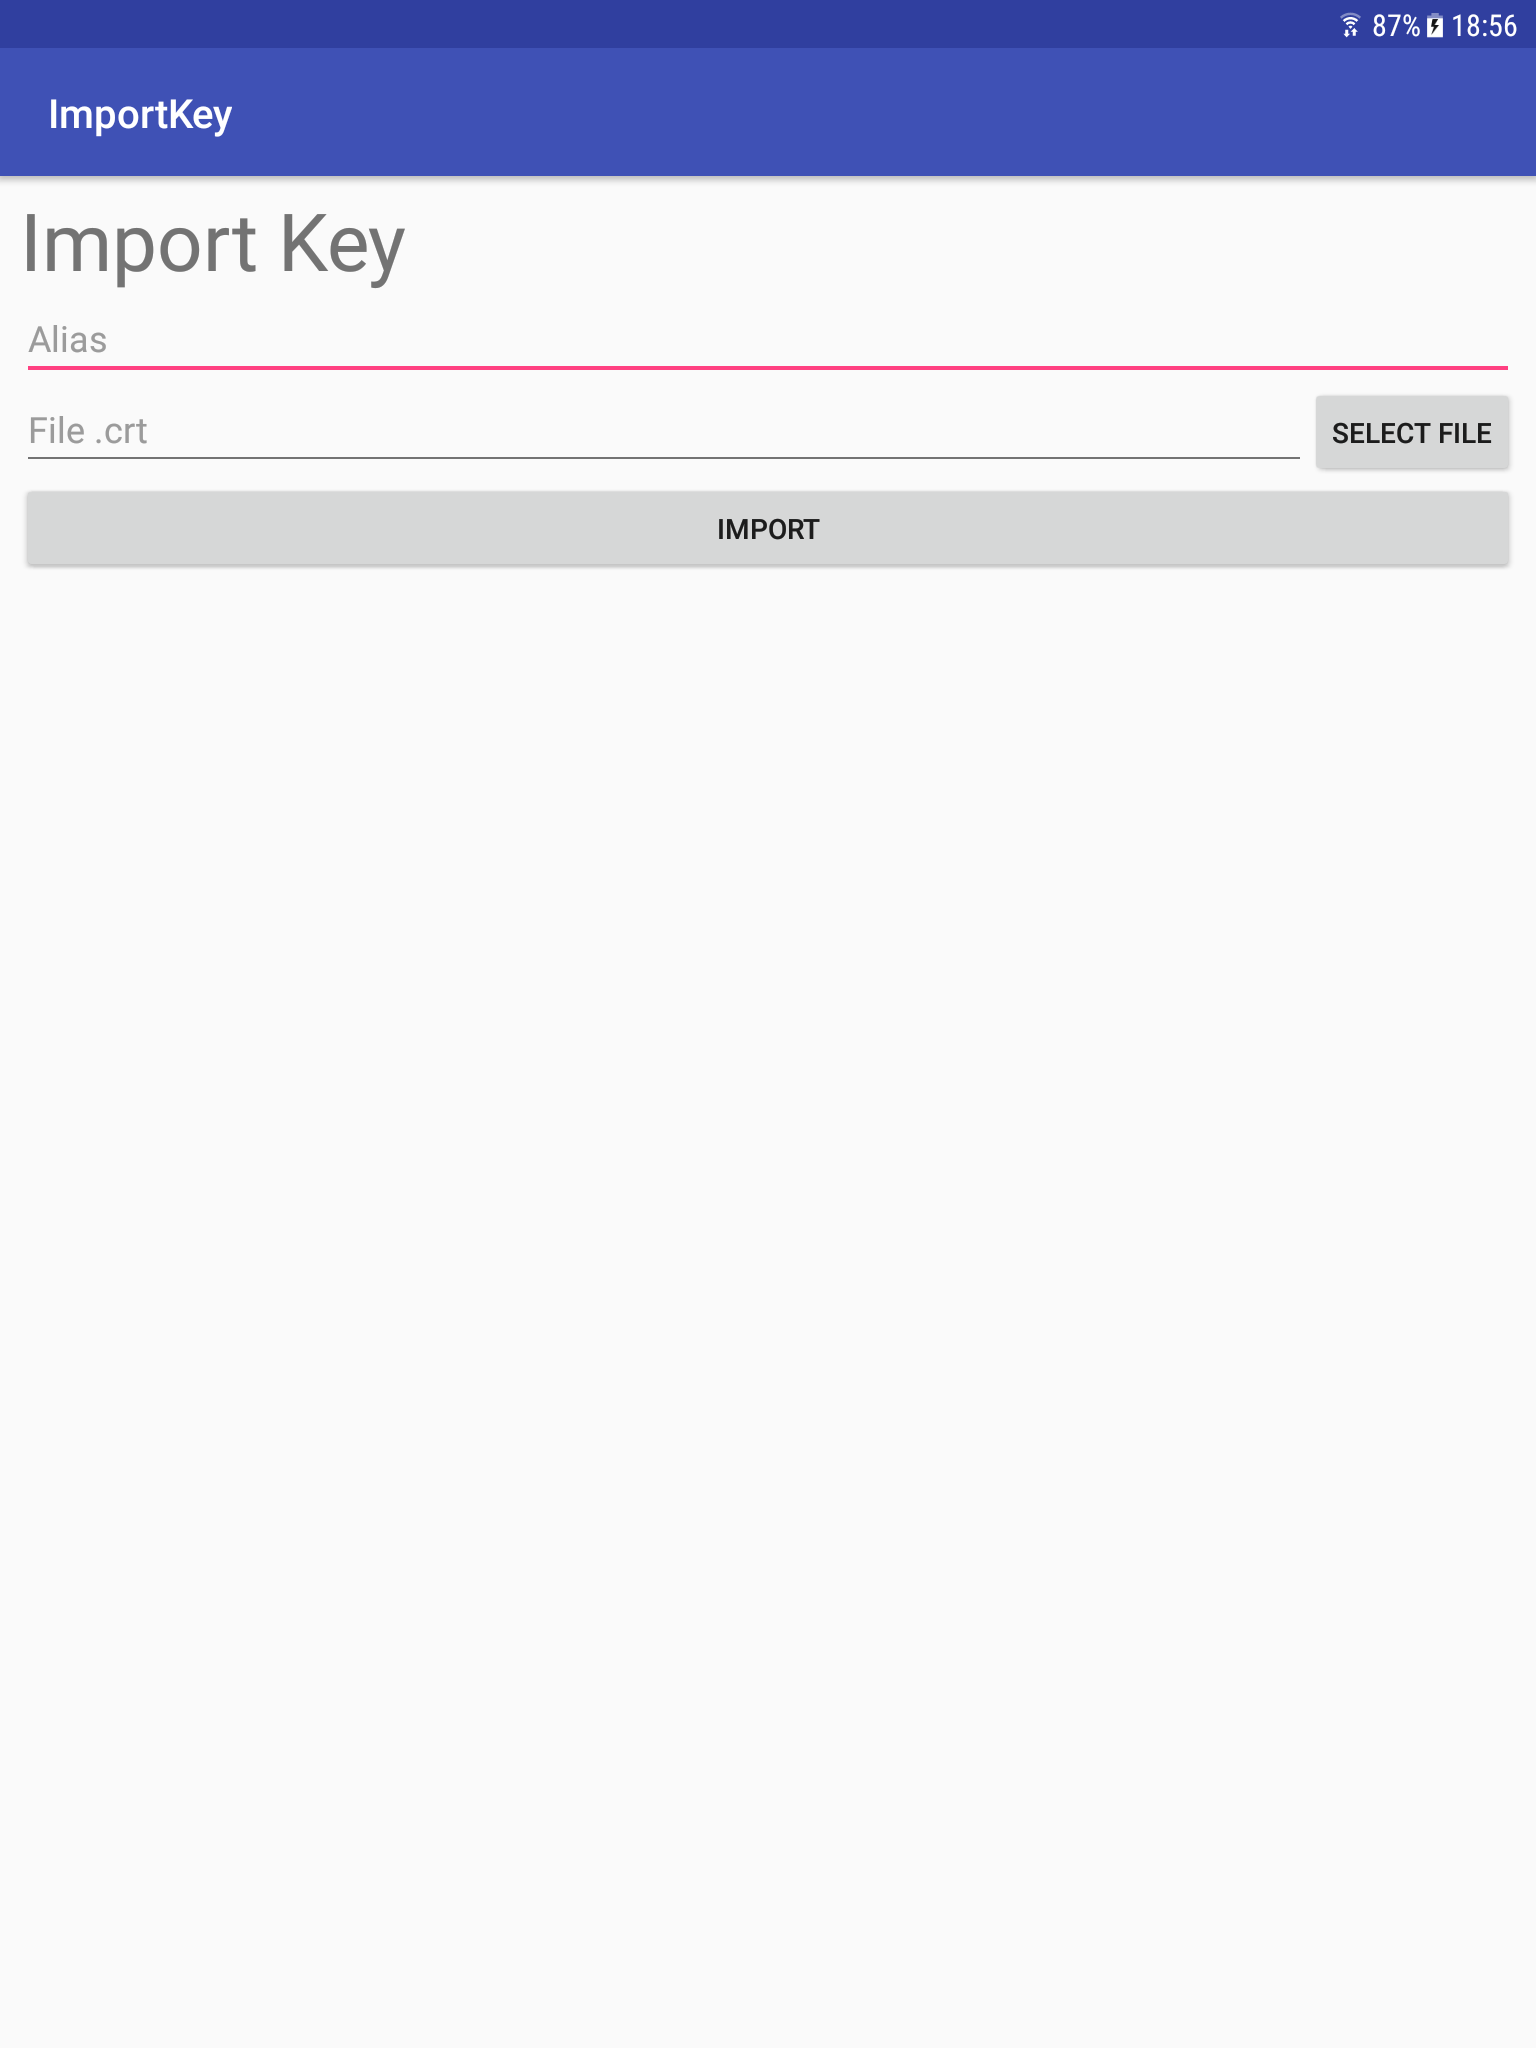
\includegraphics[scale=0.4]{Figures/import}
  \decoRule
  \caption[Shatter (Importar clave pública)]{Pantalla para importar la clave pública de un nuevo usuario}
  \label{fig:import}
\end{figure}

%De la misma manera, el nuevo contacto debe importar el certificado antes generado para poder llevar a cabo comunicaciones seguras.

Una vez el nuevo usuario se ha importado, la pantalla principal se actualiza y muestra el alias que tiene asignado, junto a unos botones con los que se puede operar con su clave pública. (Figura~\ref{fig:home_2})

\begin{figure}[!htb]
  \centering
  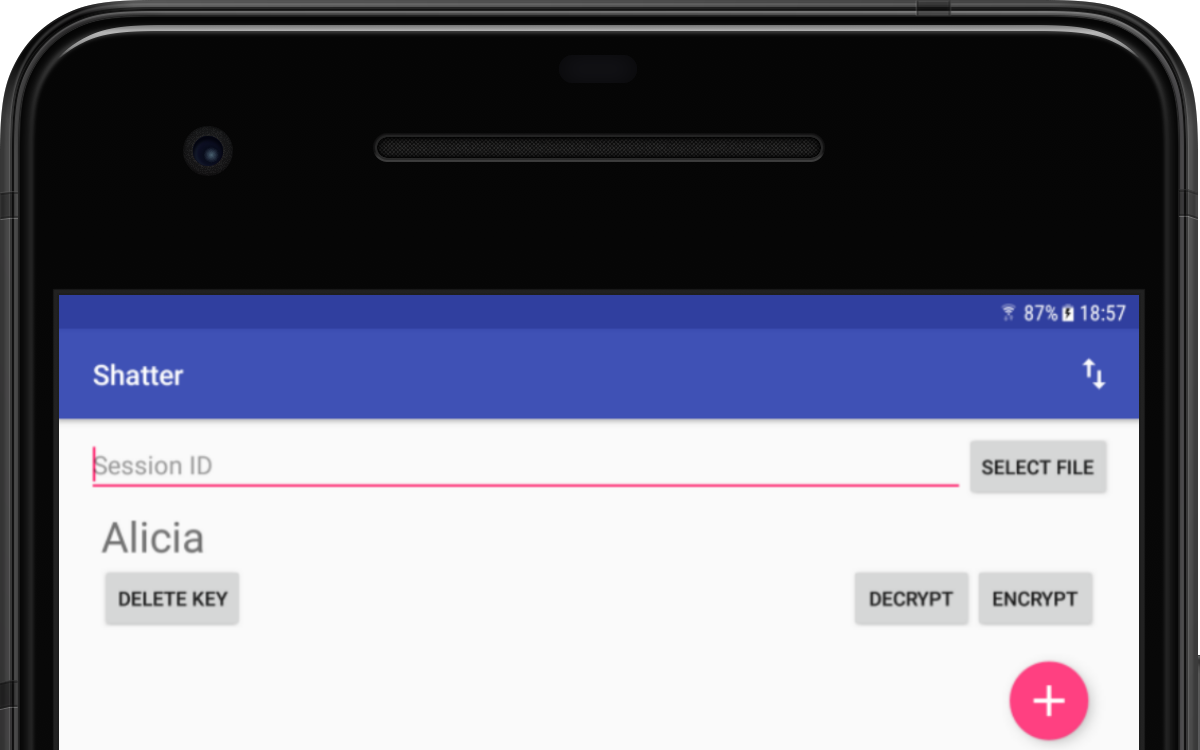
\includegraphics[scale=0.4]{Figures/home_2}
  \decoRule
  \caption[Shatter (Pantalla principal con usuarios)]{Pantalla principal de la aplicación con usuarios añadidos}
  \label{fig:home_2}
\end{figure}

\subsection{Cifrado y envío}

Para enviar un mensaje a un contacto, se debe utilizar el botón \keyword{\emph{Select File}}, el cual abre una nueva pantalla para elegir un fichero (Figura~\ref{fig:file_picker}). El selector de ficheros pone en el campo de texto de la pantalla principal el path absoluto del fichero seleccionado (también se puede escribir a mano), y ya solo queda tocar el botón \keyword{\emph{Encrypt}} del usuario al que vaya destinado el mensaje para que el fichero se fragmente y encripte. Si todo ha salido bien, se puede ver un mensaje en pantalla informando de ello, y en la ruta \path{Shatter/send/ID} se encuentran los fragmentos junto con la clave. (Figura~\ref{fig:encfiles})

\begin{figure}[!htb]
  \centering
  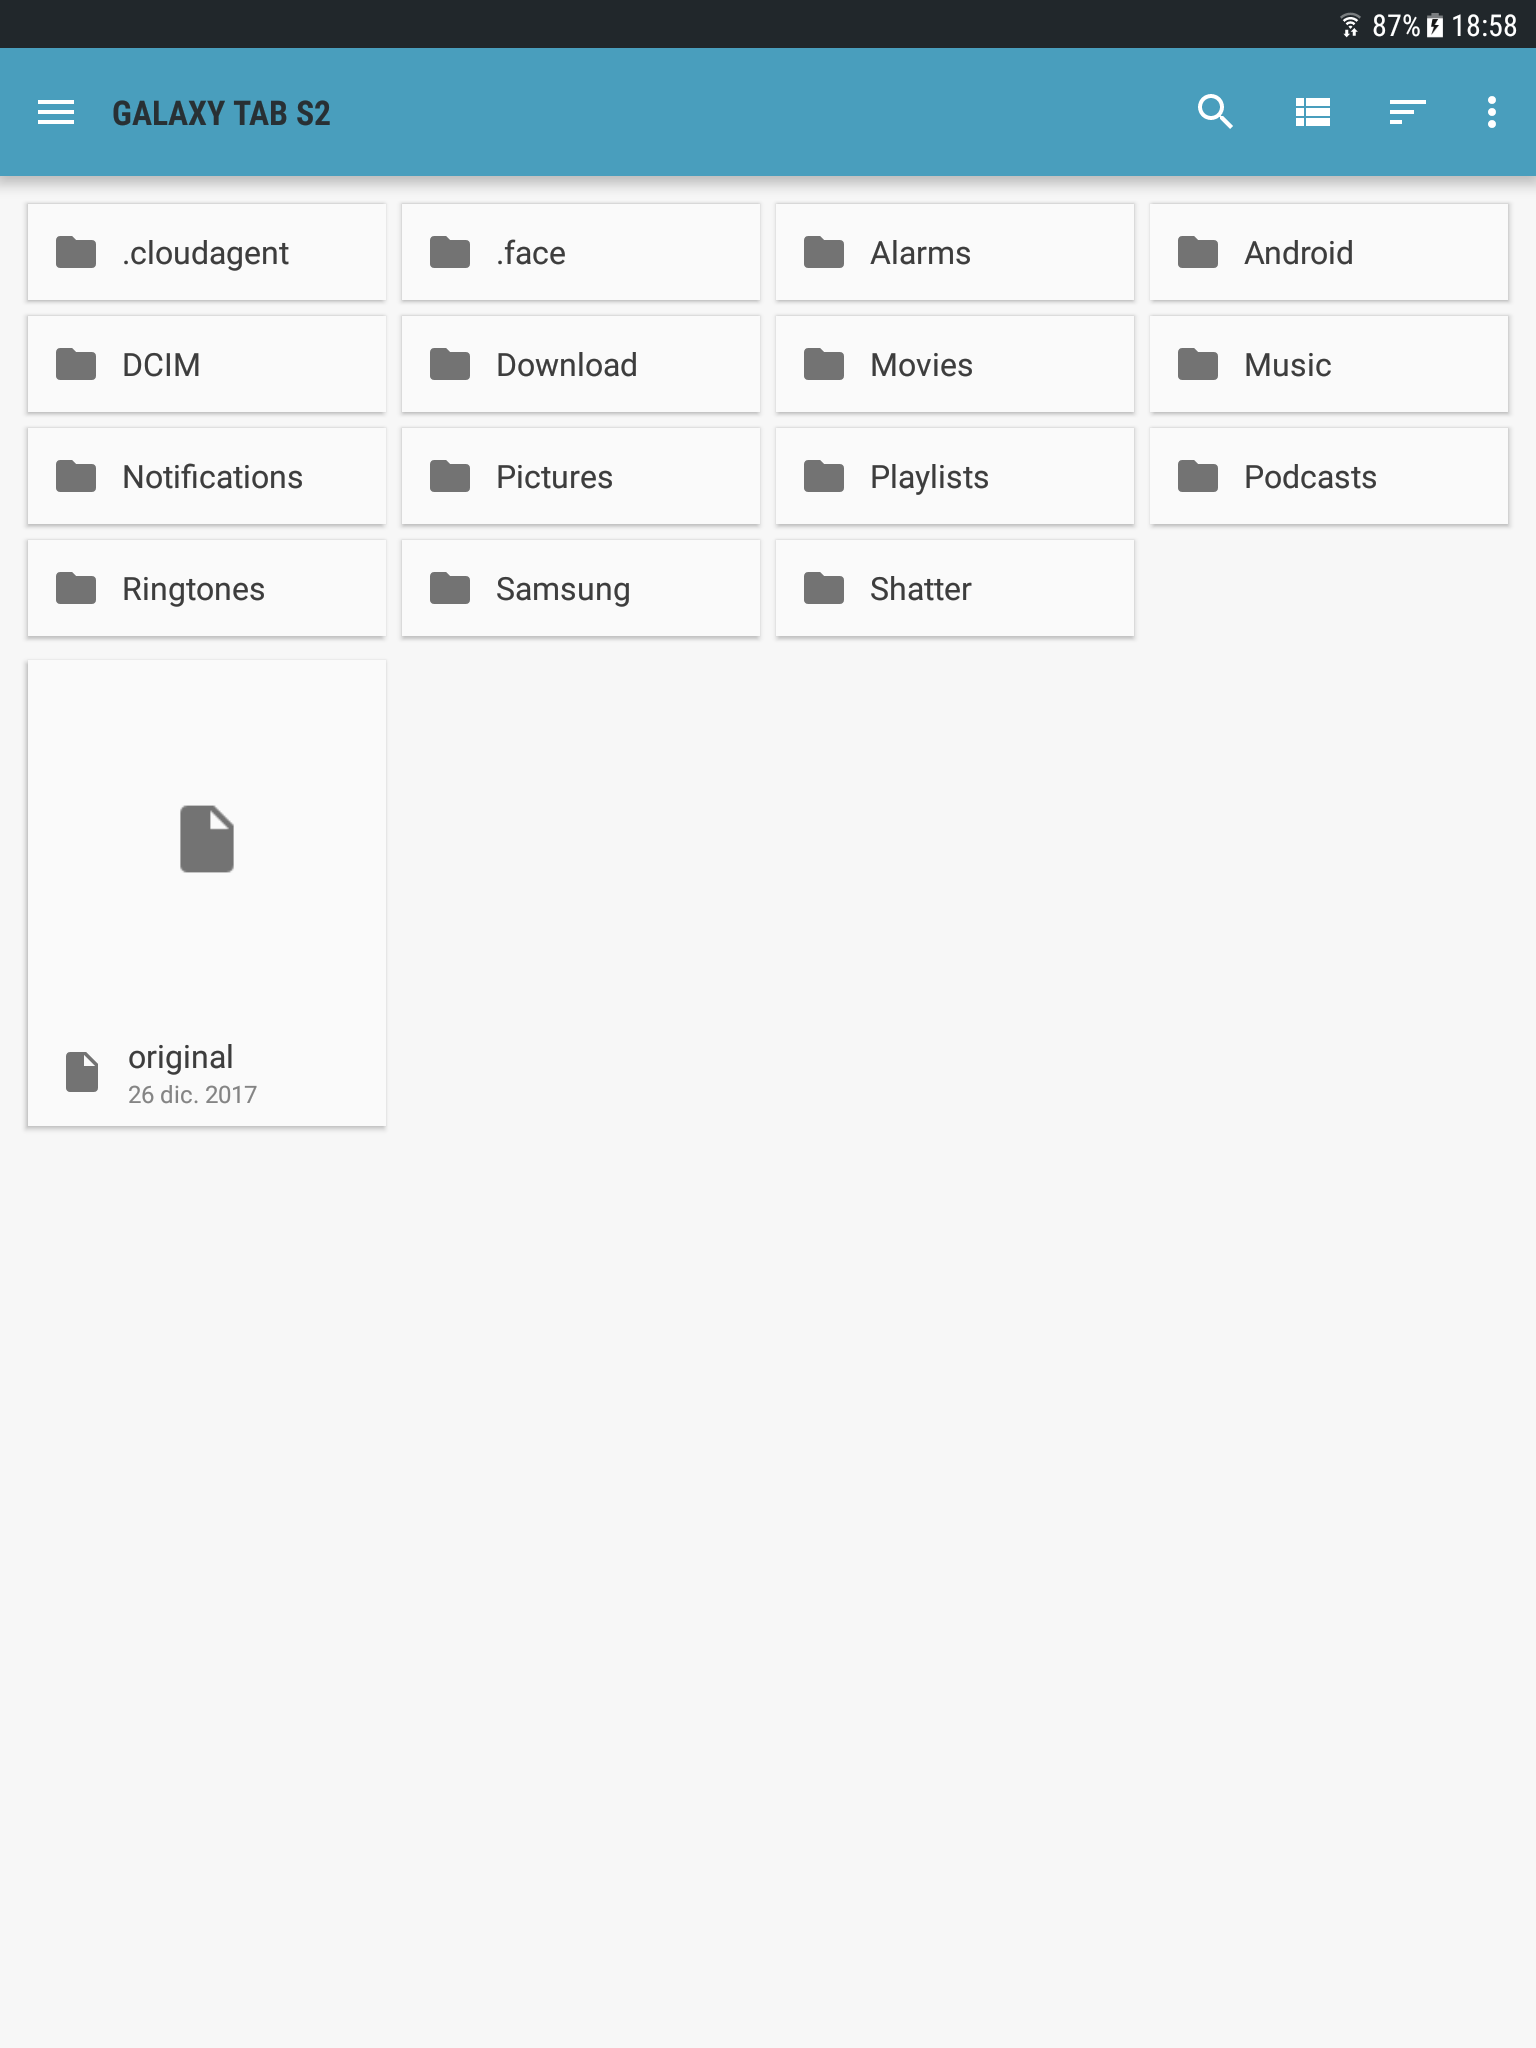
\includegraphics[scale=0.4]{Figures/file_picker}
  \decoRule
  \caption[Shatter (File Picker)]{Pantalla para seleccionar un fichero}
  \label{fig:file_picker}
\end{figure}

\begin{figure}[!htb]
  \centering
  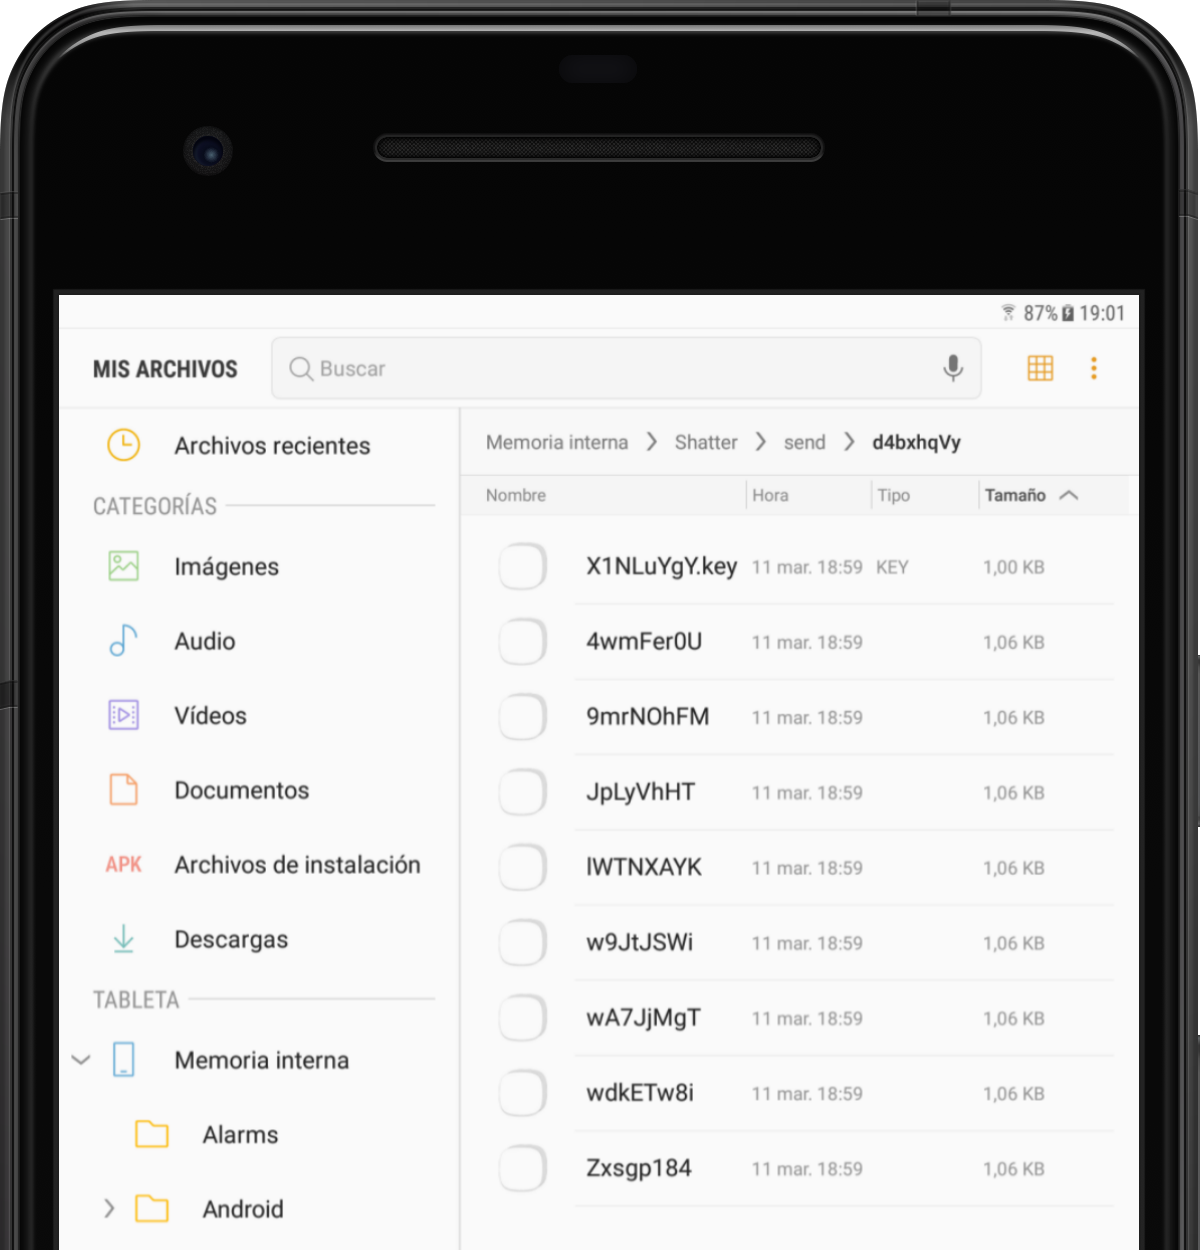
\includegraphics[scale=0.4]{Figures/encfiles}
  \decoRule
  \caption[Shatter (Mensaje fragmentado)]{Fragmentos de un mensaje junto a su clave}
  \label{fig:encfiles}
\end{figure}

El ID generado se debe comunicar al contacto al que vaya destinado, pero antes se debe subir el directorio que contiene los fragmentos al servidor haciendo uso del comando scp de Linux, por lo que se debe disponer de un usuario habilitado en la máquina que aloja el servidor. \footnote{En caso de estar encriptando el mismo mensaje para varios usuarios, se puede saber que ID corresponde a cada usuario mirando un registro que se encuentra en la ruta \path{Shatter/list.txt}}

\lstset{basicstyle=\ttfamily}
\begin{lstlisting}[language=bash]
  $ scp Shatter/send/ID server
\end{lstlisting}

\subsection{Descarga y descifrado}

Para descargar un mensaje de un contacto determinado, este debe comunicar de alguna manera el ID del mensaje, el cual se debe escribir en el campo de texto de la pantalla principal. A continuación se pulsa el botón \keyword{\emph{Decrypt}} asociado al alias del contacto.
%Si nuestro contacto quisiera descargarse el mensaje, escribirá el ID que le comunicamos antes en el campo de texto de la pantalla principal. Como sabe que el mensaje viene de nuestra parte, tocará el botón \emph{Decrypt} de nuestra clave pública.

Con esto, la aplicación pide al servidor un índice con todos los ficheros asociados a ese ID y descarga todos los que pueda en el directorio \path{Shatter/ID}. En caso de que algún fichero falte, informa de ello al usuario antes de proceder con el descifrado y rellena un registro indicando cuales son los fragmentos que faltan. (Figura~\ref{fig:miss})

\begin{figure}[!htb]
  \centering
  
\includegraphics[scale=0.4]{Figures/miss}
  \decoRule
  \caption[Shatter (Faltan fragmentos)]{Mensaje advirtiendo de que algunos fragmentos no se han descargado}
  \label{fig:miss}
\end{figure}

Si todos los fragmentos y la clave son descargados exitosamente, la aplicación procede con el descifrado de los mismos. Durante el proceso se crean, en caso de ser necesario, ficheros de registro en los cuales se reflejan los problemas surgidos. En caso de no ocurrir ningún problema, el fichero original se recompone en la ruta \path{Shatter/ID/done/ID}. (Figura~\ref{fig:done})

\begin{figure}[!htb]
  \centering
  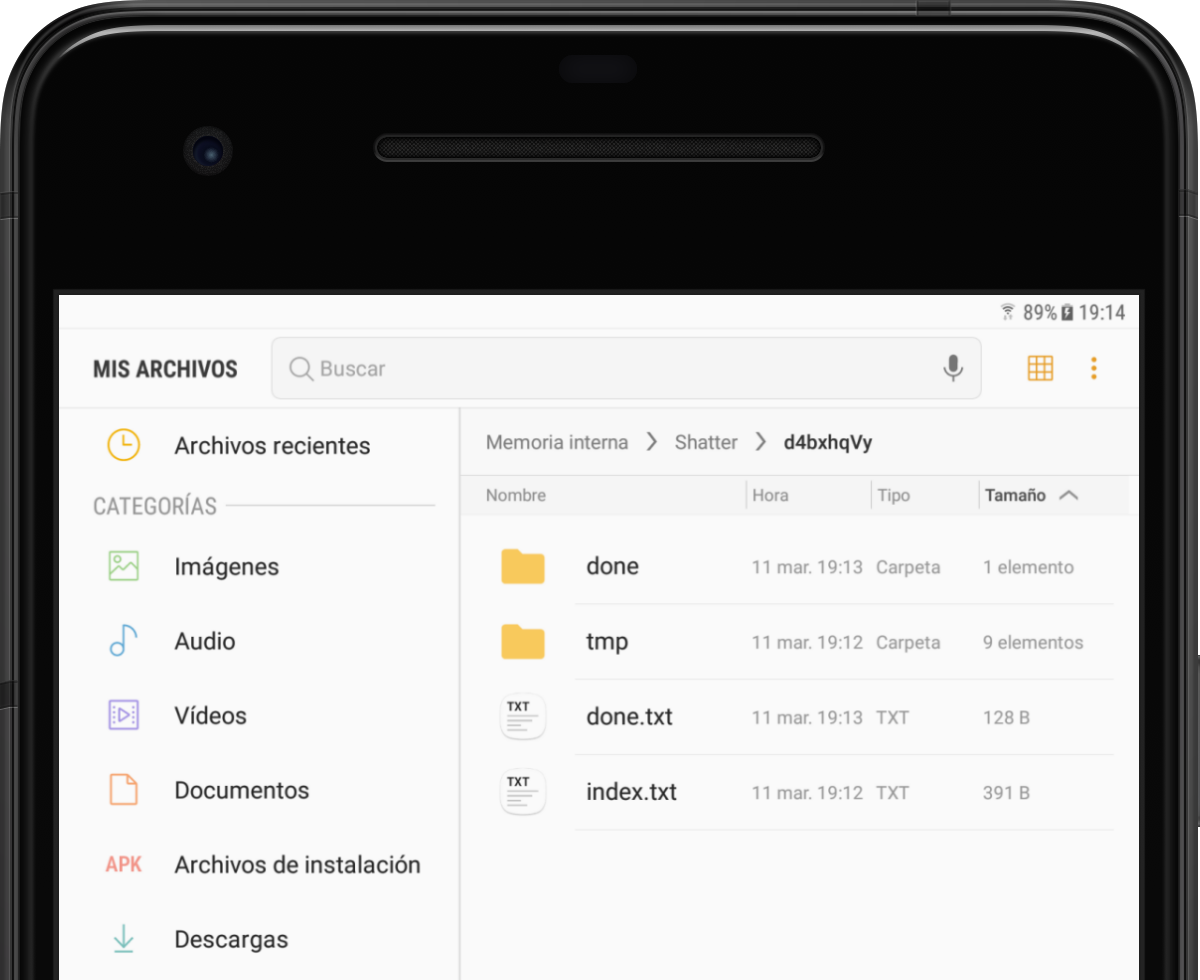
\includegraphics[scale=0.4]{Figures/done}
  \decoRule
  \caption[Shatter (Mensaje recibido)]{Directorio de un mensaje recibido}
  \label{fig:done}
\end{figure}

%-------------------------------------------------------------------------------

\section{Problemas encontrados}

A lo largo de la etapa que supuso el desarrollo de la aplicación, se han encontrado varios problemas que dificultaron la finalización del proyecto.

El mayor problema con el que se tuvo que lidiar es el no haber creado una parte portable que hiciera más fácil la migración a Android. Algunas librerías usadas cuando el proyecto solo era una aplicación escrita en Java tienen ciertas dependencias, las cuales no se encuentran en ninguna librería Java usada en Android. Además, el uso del Keystore de Android para almacenar las claves exige realizar el cifrado asimétrico, las firmas y la generación de las claves de una manera determinada, lo que supuso la eliminación de las clases que se encargaban anteriormente de ello (RSALibrary y RSAPSS). Aunque algunos de estos problemas no se habrían podido solucionar aun teniendo una parte portable, sin duda habría supuesto un ahorro considerable de tiempo.

A raíz de lo anterior, la mayoría de las clases no estuvieron bien definidas desde un principio. Esto supuso muchos cambios a lo largo del desarrollo de la aplicación (Cabeceras, modos de cifrado, registros...). De nuevo, una buena planificación habría ahorrado una gran cantidad de tiempo y energía.

Pero no todos los problemas encontrados tienen que ver con la desorganización. La aplicación ahora cuenta con un servidor dedicado pero, en un principio, se pensó en utilizar un servicio externo para el almacenamiento de los mensajes enviados por los usuarios. De algunas ideas que salieron, se eligió la aplicación Pastebin\footnote{\url{https://pastebin.com/}}, ya que permite la subida anónima de texto plano. La idea era que la aplicación subiera los distintos fragmentos cifrados a la plataforma, permitiendo al resto de usuarios su descarga. Sin embargo, la existencia de límites en el número de mensajes enviados o en la longitud de los mismos hicieron que se desechara la idea en favor de un servidor dedicado.

%% Chapter 6: Last Conclusions

\chapter{Conclusiones finales} % Main chapter title

\label{Chapter6} % Reference

%----------------------------------------------------------------------------------------

\section{Objetivos alcanzados}

%----------------------------------------------------------------------------------------

\section{Líneas futuras}


%----------------------------------------------------------------------------------------
%	THESIS CONTENT - APPENDICES
%----------------------------------------------------------------------------------------

\appendix % Cue to tell LaTeX that the following "chapters" are Appendices

% Include the appendices of the thesis as separate files from the Appendices folder
% Uncomment the lines as you write the Appendices

% Appendix A

\chapter{Frequently Asked Questions} % Main appendix title

\label{AppendixA} % For referencing this appendix elsewhere, use \ref{AppendixA}

\section{How do I change the colors of links?}

The color of links can be changed to your liking using:

{\small\verb!\hypersetup{urlcolor=red}!}, or

{\small\verb!\hypersetup{citecolor=green}!}, or

{\small\verb!\hypersetup{allcolor=blue}!}.

\noindent If you want to completely hide the links, you can use:

{\small\verb!\hypersetup{allcolors=.}!}, or even better: 

{\small\verb!\hypersetup{hidelinks}!}.

\noindent If you want to have obvious links in the PDF but not the printed text, use:

{\small\verb!\hypersetup{colorlinks=false}!}.

%\include{Appendices/AppendixB}
%\include{Appendices/AppendixC}

%----------------------------------------------------------------------------------------
%	BIBLIOGRAPHY
%----------------------------------------------------------------------------------------

\printbibliography[heading=bibintoc]

%----------------------------------------------------------------------------------------

\end{document}
